% datastruct/datastruct.tex
% mainfile: ../perfbook.tex
% SPDX-License-Identifier: CC-BY-SA-3.0

\QuickQuizChapter{chp:Data Structures}{Data Structures}{qqzdatastruct}
%
\Epigraph{Bad programmers worry about the code.
	  Good programmers worry about data structures and their
	  relationships.}
	 {Linus Torvalds}

Serious discussions of algorithms include time complexity of their
data structures~\cite{ThomasHCorman2001Algorithms}.
However, for parallel programs, the time complexity includes concurrency
effects because these effects can be overwhelmingly large, as shown in
\cref{chp:Hardware and its Habits}.
In other words, a good programmer's data-structure relationships
include those aspects related to concurrency.

This chapter will expose a number of complications:

\begin{enumerate}
\item	Data structures designed in full accordance with the
	good advice given in
	\cref{chp:Partitioning and Synchronization Design}
	can nonetheless abjectly fail to scale on some types of systems.
\label{sec:datastruct:NUMA-induced failure to scale}
\item	Data structures designed in full accordance with the
	good advice given in both
	\cref{chp:Partitioning and Synchronization Design}
	and
	\cref{chp:Deferred Processing}
	can \emph{still} abjectly fail to scale on some types of systems.
\label{sec:datastruct:Cache-size-induced failure to scale}
\item	Even \emph{read-only synchronization-free} data-structure traversal 
	can fail to scale on some types of systems.
\label{sec:datastruct:Cache-size-induced failure to scale redux}
\item	Data-structure traversals avoiding the aforementioned complications
	can still be impeded by concurrent updates.
\label{sec:datastruct:Update-activity failure to scale}
\end{enumerate}

This chapter will investigate these complications and demostrate some
ways of unraveling them.

\Cref{sec:datastruct:Motivating Application}
presents the motivating application for this chapter's data structures.
\Cref{chp:Partitioning and Synchronization Design} showed how
partitioning improves scalability, so
\cref{sec:datastruct:Partitionable Data Structures}
discusses partitionable data structures.
\Cref{chp:Deferred Processing} described how deferring some
actions can greatly improve both performance and scalability,
a topic taken up by
\cref{sec:datastruct:Read-Mostly Data Structures}.
\Cref{sec:datastruct:Non-Partitionable Data Structures}
looks at a non-partitionable data structure, splitting
it into read-mostly and partitionable portions,
which improves both performance and scalability.
Because this chapter cannot delve into the details of every concurrent
data structure,
\cref{sec:datastruct:Other Data Structures}
surveys a few of the important ones.
Finally, \cref{sec:datastruct:Summary}
presents a summary of this chapter.

\section{Motivating Application}
\label{sec:datastruct:Motivating Application}
%
\epigraph{The art of doing mathematics consists in finding that special
	  case which contains all the germs of generality.}
	 {David Hilbert}

We will use the Schr\"odinger's Zoo application to evaluate
performance~\cite{McKenney:2013:SDS:2483852.2483867}.
Schr\"odinger has a zoo containing a large number of animals, and
he would like to track them using an in-memory database with
each animal in the zoo represented by a data item in this database.
Each animal has a unique name that is used as a key, with a variety
of data tracked for each animal.

Births, captures, and purchases result in insertions, while deaths,
releases, and sales result in deletions.
Because Schr\"odinger's zoo contains a large quantity of short-lived
animals, including mice and insects, the database must handle
high update rates.
Those interested in Schr\"odinger's animals can query them, and
Schr\"odinger has noted suspiciously query rates for his cat, so much
so that he suspects that his mice might be checking up on their nemesis.
Whatever their source, Schr\"odinger's application must handle high
query rates to a single data element.

As we will see, this simple application can pose a challenge to
traditional concurrent data structures.

\section{Partitionable Data Structures}
\label{sec:datastruct:Partitionable Data Structures}
%
\epigraph{Finding a way to live the simple life today is the most
	  complicated task.}
	 {Henry A. Courtney, updated}

There are a huge number of data structures in use today, so much so
that there are multiple textbooks covering them.
This section focuses on a single data structure, namely the hash table.
This focused approach allows a much deeper investigation of how concurrency
interacts with data structures, and also focuses on a data structure
that is heavily used in practice.
\Cref{sec:datastruct:Hash-Table Design}
overviews the design, and
\cref{sec:datastruct:Hash-Table Implementation}
presents the implementation.
Finally,
\cref{sec:datastruct:Hash-Table Performance}
discusses the resulting performance and scalability.

\subsection{Hash-Table Design}
\label{sec:datastruct:Hash-Table Design}

\Cref{chp:Partitioning and Synchronization Design}
emphasized the need to apply partitioning in order to attain
respectable performance and scalability, so partitionability
must be a first-class criterion when selecting data structures.
This criterion is well satisfied by that workhorse of parallelism,
the hash table.
Hash tables are conceptually simple, consisting of an array of
\emph{hash buckets}.
A \emph{hash function} maps from a given element's \emph{key}
to the hash bucket that this element will be stored in.
Each hash bucket therefore heads up a linked list of elements,
called a \emph{hash chain}.
When properly configured, these hash chains will be quite short,
permitting a hash table to access its elements extremely efficiently.

\QuickQuiz{
	But chained hash tables are but one type of many.
	Why the focus on chained hash tables?
}\QuickQuizAnswer{
	Chained hash tables are completely partitionable, and thus
	well-suited to concurrent use.
	There are other completely-partitionable hash tables, for
	example, split-ordered list~\cite{OriShalev2006SplitOrderListHash},
	but they are considerably more complex.
	We therefore focus on chained hash tables.
}\QuickQuizEnd

In addition, each bucket has its own lock, so that elements in different
buckets of the hash table may be added, deleted, and looked up completely
independently.
A large hash table with a large number of buckets (and thus locks), with
each bucket containing a small number of elements should therefore provide
excellent scalability.

This approach solves the element-count issue called out in
\cref{sec:intro:Existing Sequential Designs}
by refraining from returning any count of the number of elements in
the hash table from either \co{hashtab_add()} or \co{hashtab_del()}.
It further simplifies the API by allowing duplicate elements and by
passing a pointer to the element to be deleted to \co{hashtab_del()}.
These two changes eliminate the possibility of error returns, which
means that the \co{hashtab_add()} and \co{hashtab_del()} functions'
return types can be \co{void}.

\subsection{Hash-Table Implementation}
\label{sec:datastruct:Hash-Table Implementation}

\begin{fcvref}[ln:datastruct:hash_bkt:struct]
\Cref{lst:datastruct:Hash-Table Data Structures}
(\path{hash_bkt.c})
shows a set of data structures used in a simple fixed-sized hash
table using chaining and per-hash-bucket locking, and
\cref{fig:datastruct:Hash-Table Data-Structure Diagram}
diagrams how they fit together.
Note that the \co{cds_} functions and data structures may be found
in the userspace RCU
library~\cite{MathieuDesnoyers2009URCU,PaulMcKenney2013LWNURCUqueuestack,PaulMcKenney2013LWNURCUqueuestackAPI,PaulMcKenney2013LWNURCUlist}.
The \co{hashtab} structure (\clnrefrange{tab:b}{tab:e} in
\cref{lst:datastruct:Hash-Table Data Structures})
contains four \co{ht_bucket} structures
(\clnrefrange{bucket:b}{bucket:e} in
\cref{lst:datastruct:Hash-Table Data Structures}),
with the \co{->ht_nbuckets} field controlling the number of buckets
and the \co{->ht_cmp} field holding the pointer to key-comparison
function.
Each such bucket contains a list header \co{->htb_head} and
a lock \co{->htb_lock}.
The list headers chain \co{ht_elem} structures
(\clnrefrange{elem:b}{elem:e} in
\cref{lst:datastruct:Hash-Table Data Structures})
through their
\co{->hte_next} fields, and each \co{ht_elem} structure also caches
the corresponding element's hash value in the \co{->hte_hash} field.
The \co{ht_elem} structure is included in a larger structure
which might contain a complex key.
\end{fcvref}
\Cref{fig:datastruct:Hash-Table Data-Structure Diagram}
shows bucket~0 containing two elements and bucket~2 containing one.

\begin{listing}
\input{CodeSamples/datastruct/hash/hash_bkt@struct.fcv}
\caption{Hash-Table Data Structures}
\label{lst:datastruct:Hash-Table Data Structures}
\end{listing}

\begin{figure}
\centering
\resizebox{3in}{!}{\includegraphics{datastruct/hashdiagram}}
\caption{Hash-Table Data-Structure Diagram}
\label{fig:datastruct:Hash-Table Data-Structure Diagram}
\end{figure}

\begin{fcvref}[ln:datastruct:hash_bkt:map_lock:map]
\Cref{lst:datastruct:Hash-Table Mapping and Locking}
shows mapping and locking functions.
\Clnref{b,e}
show the macro \co{HASH2BKT()}, which maps from a hash value
to the corresponding \co{ht_bucket} structure.
This macro uses a simple modulus:
If more aggressive hashing is required,
the caller needs to implement it when mapping from key to hash value.
The remaining two functions acquire and release the \co{->htb_lock}
corresponding to the specified hash value.
\end{fcvref}

\begin{listing}
\input{CodeSamples/datastruct/hash/hash_bkt@map_lock.fcv}
\caption{Hash-Table Mapping and Locking}
\label{lst:datastruct:Hash-Table Mapping and Locking}
\end{listing}

\begin{fcvref}[ln:datastruct:hash_bkt:lookup]
\Cref{lst:datastruct:Hash-Table Lookup}
shows \co{hashtab_lookup()},
which returns a pointer to the element with the specified hash and key,
or \co{NULL} if that element does not exist.
This function takes both a hash value and a pointer to the key because
this allows users of this function to use arbitrary keys and
arbitrary hash functions.
\Clnref{map} maps from the hash value to a pointer to the corresponding
hash bucket.
Each pass through the loop spanning
\clnrefrange{loop:b}{loop:e} examines one element
of the bucket's hash chain.
\Clnref{hashmatch} checks to see if the hash values match, and if not,
\clnref{next}
proceeds to the next element.
\Clnref{keymatch} checks to see if the actual key matches, and if so,
\clnref{return} returns a pointer to the matching element.
If no element matches, \clnref{ret_NULL} returns \co{NULL}.
\end{fcvref}

\begin{listing}
\input{CodeSamples/datastruct/hash/hash_bkt@lookup.fcv}
\caption{Hash-Table Lookup}
\label{lst:datastruct:Hash-Table Lookup}
\end{listing}

\QuickQuiz{
	\begin{fcvref}[ln:datastruct:hash_bkt:lookup]
	But isn't the double comparison on
	\clnrefrange{hashmatch}{return} in
	\cref{lst:datastruct:Hash-Table Lookup} inefficient
	in the case where the key fits into an unsigned long?
	\end{fcvref}
}\QuickQuizAnswer{
	Indeed it is!
	However, hash tables quite frequently store information with
	keys such as character strings that do not necessarily fit
	into an unsigned long.
	Simplifying the hash-table implementation for the case where
	keys always fit into unsigned longs is left as an exercise
	for the reader.
}\QuickQuizEnd

\begin{listing}
\input{CodeSamples/datastruct/hash/hash_bkt@add_del.fcv}
\caption{Hash-Table Modification}
\label{lst:datastruct:Hash-Table Modification}
\end{listing}

\Cref{lst:datastruct:Hash-Table Modification}
shows the \co{hashtab_add()} and \co{hashtab_del()} functions
that add and delete elements from the hash table, respectively.

\begin{fcvref}[ln:datastruct:hash_bkt:add_del:add]
The \co{hashtab_add()} function simply sets the element's hash
value on \clnref{set}, then adds it to the corresponding bucket on
\clnref{add:b,add:e}.
\end{fcvref}
The \co{hashtab_del()} function simply removes the specified element
from whatever hash chain it is on, courtesy of the doubly linked
nature of the hash-chain lists.
Before calling either of these two functions, the caller is required to
ensure that no other thread is accessing
or modifying this same bucket, for example, by invoking
\co{hashtab_lock()} beforehand.

\begin{listing}
\input{CodeSamples/datastruct/hash/hash_bkt@alloc_free.fcv}
\caption{Hash-Table Allocation and Free}
\label{lst:datastruct:Hash-Table Allocation and Free}
\end{listing}

\Cref{lst:datastruct:Hash-Table Allocation and Free}
shows \co{hashtab_alloc()} and \co{hashtab_free()},
which do hash-table allocation and freeing, respectively.
\begin{fcvref}[ln:datastruct:hash_bkt:alloc_free:alloc]
Allocation begins on
\clnrefrange{alloc:b}{alloc:e} with allocation of the underlying memory.
If \clnref{chk_NULL} detects that memory has been exhausted,
\clnref{ret_NULL} returns
\co{NULL} to the caller.
Otherwise, \clnref{set_nbck,set_cmp} initialize
the number of buckets and the pointer to key-comparison function,
and the loop
spanning \clnrefrange{loop:b}{loop:e} initializes the buckets themselves,
including the chain list header on
\clnref{init_head} and the lock on \clnref{init_lock}.
Finally, \clnref{return} returns a pointer to the newly allocated hash table.
\end{fcvref}
\begin{fcvref}[ln:datastruct:hash_bkt:alloc_free:free]
The \co{hashtab_free()} function on
\clnrefrange{b}{e} is straightforward.
\end{fcvref}

\subsection{Hash-Table Performance}
\label{sec:datastruct:Hash-Table Performance}

\begin{figure}
\centering
\resizebox{2.5in}{!}{\includegraphics{CodeSamples/datastruct/hash/data/hps.perf.2020.11.26a/zoocpubktlin8}}
\caption{Read-Only Hash-Table Performance For Schr\"odinger's Zoo}
\label{fig:datastruct:Read-Only Hash-Table Performance For Schroedinger's Zoo}
\end{figure}

The performance results for a single 28-core socket of a 2.1\,GHz
Intel Xeon system using a bucket-locked hash table
with 262,144 buckets are shown in
\cref{fig:datastruct:Read-Only Hash-Table Performance For Schroedinger's Zoo}.
The performance does scale nearly linearly, but falls far short ideal,
even at only 28~CPUs.
Part of this shortfall is due to the fact that lock acquisitions and
releases incur communications cache misses only on two or more CPUs.

\begin{figure}
\centering
\resizebox{2.5in}{!}{\includegraphics{CodeSamples/datastruct/hash/data/hps.perf.2020.11.26a/zoocpubktlin}}
\caption{Read-Only Hash-Table Performance For Schr\"odinger's Zoo, 448 CPUs}
\label{fig:datastruct:Read-Only Hash-Table Performance For Schroedinger's Zoo; 448 CPUs}
\end{figure}

And things only get worse with more CPUs, as can be seen in
\cref{fig:datastruct:Read-Only Hash-Table Performance For Schroedinger's Zoo; 448 CPUs}.
We do not need to show ideal performance:
The performance for 29~CPUs and beyond is abysmal.
This clearly underscores the dangers of extrapolating performance from a
modest number of CPUs.

Of course, one possible reason for the collapse in performance might be
that more hash buckets are needed.
We can test this by increasing the number of hash buckets.

\QuickQuiz{
	Instead of simply increasing the number of hash buckets,
	wouldn't it be better to cache-align the existing hash buckets?
}\QuickQuizAnswer{
	The answer depends on a great many things.
	If the hash table has a large number of elements per bucket, it
	would clearly be better to increase the number of hash buckets.
	On the other hand, if the hash table is lightly loaded,
	the answer depends on the hardware, the effectiveness of the
	hash function, and the workload.
	Interested readers are encouraged to experiment.
}\QuickQuizEnd


\begin{figure}
\centering
\resizebox{2.5in}{!}{\includegraphics{CodeSamples/datastruct/hash/data/hps.perf.2020.11.26a/zoocpubktsizelin}}
\caption{Read-Only Hash-Table Performance For Schr\"odinger's Zoo, Varying Buckets}
\label{fig:datastruct:Read-Only Hash-Table Performance For Schroedinger's Zoo; Varying Buckets}
\end{figure}

However, as can be seen in
\cref{fig:datastruct:Read-Only Hash-Table Performance For Schroedinger's Zoo; Varying Buckets},
changing the number of buckets has almost no effect:
Scalability is still abysmal.
In particular, we still see a sharp dropoff at 29~CPUs and beyond,
clearly demonstrating the complication put forward by
\cref{sec:datastruct:NUMA-induced failure to scale}
of the list of complications on
\cpageref{sec:datastruct:NUMA-induced failure to scale}.
Clearly, something else is going on.

The problem is that this is a multi-socket system, with CPUs~0--27
and~224--251 mapped to the first socket as shown in
\cref{fig:datastruct:NUMA Topology of System Under Test}.
Test runs confined to the first 28~CPUs therefore perform quite
well, but tests that involve socket~0's CPUs~0--27 as well as
socket~1's CPU~28 incur the overhead of passing data across
socket boundaries.
This can severely degrade performance, as was discussed in
\cref{sec:cpu:Hardware System Architecture}.
In short, large multi-socket systems require good locality of reference
in addition to full partitioning.
The remainder of this chapter will discuss ways of providing good
locality of reference within the hash table itself, but in the
meantime please note that one other way to provide good locality
of reference would be to place large data elements in the hash
table.
For example, Schr\"odinger might attain excellent cache locality by
placing photographs or even videos of his animals in each element of
the hash table.
But for those needing hash tables containing small data elements,
please read on!

\QuickQuiz{
	Given the negative scalability of the Schr\"odinger's
	Zoo application across sockets, why not just run multiple
	copies of the application, with each copy having a subset
	of the animals and confined to run on a single socket?
}\QuickQuizAnswer{
	You can do just that!
	In fact, you can extend this idea to large clustered systems,
	running one copy of the application on each node of the cluster.
	This practice is called ``sharding'', and is heavily used in
	practice by large web-based
	retailers~\cite{DeCandia:2007:DAH:1323293.1294281}.

	However, if you are going to shard on a per-socket basis within
	a multisocket system, why not buy separate smaller and cheaper
	single-socket systems, and then run one shard of the database
	on each of those systems?
}\QuickQuizEnd

One key property of these Schr\"odinger's-zoo experiments is they are
all read-only.
This makes the performance degradation due to lock-acquisition-induced
cache misses all the more painful.
Even though we are not updating the underlying hash table itself, we are
still paying the price for writing to memory.
Of course, if the hash table was never going to be updated, we could dispense
entirely with mutual exclusion.
This approach is quite straightforward and is left as an exercise for the
reader.
But even with the occasional update, avoiding writes avoids cache
misses, and allows the read-mostly data to be replicated across all
the caches, which in turn promotes locality of reference.

The next section therefore examines optimizations that can be carried out in
read-mostly cases where updates are rare, but could happen at any time.

\setlength\dashlinedash{1pt}
\setlength\dashlinegap{2pt}

\begin{table}
\renewcommand*{\arraystretch}{1.2}
\centering
\begin{tabular}{r||c:c}
	& \multicolumn{2}{c}{Hyperthread} \\
	\cline{2-3}
	Socket & 0 &  1 \\
	\hline
	\hline
	0 &    0--27 & 224--251 \\
	\cdashline{2-3}
	1 &   28--55 & 252--279 \\
	\cdashline{2-3}
	2 &   56--83 & 280--307 \\
	\cdashline{2-3}
	3 &  84--111 & 308--335 \\
	\cdashline{2-3}
	4 & 112--139 & 336--363 \\
	\cdashline{2-3}
	5 & 140--167 & 364--391 \\
	\cdashline{2-3}
	6 & 168--195 & 392--419 \\
	\cdashline{2-3}
	7 & 196--223 & 420--447 \\
\end{tabular}
\caption{NUMA Topology of System Under Test}
\label{fig:datastruct:NUMA Topology of System Under Test}
\end{table}

\section{Read-Mostly Data Structures}
\label{sec:datastruct:Read-Mostly Data Structures}
%
\epigraph{Adapt the remedy to the disease.}{Chinese proverb}

Although partitioned data structures can offer excellent scalability,
\IXacr{numa} effects can result in severe degradations of both performance and
scalability.
In addition,
the need for read-side synchronization can degrade performance in
read-mostly situations.
However, we can achieve both performance and scalability by using
RCU, which was introduced in
\cref{sec:defer:Read-Copy Update (RCU)}.
Similar results can be achieved using \IXpl{hazard pointer}
(\path{hazptr.c})~\cite{MagedMichael04a}, which will be included in
the performance results shown in this
section~\cite{McKenney:2013:SDS:2483852.2483867}.

\subsection{RCU-Protected Hash Table Implementation}
\label{sec:datastruct:RCU-Protected Hash Table Implementation}

For an RCU-protected hash table with per-bucket locking,
updaters use locking as shown in
\cref{sec:datastruct:Partitionable Data Structures},
but readers use RCU\@.
The data structures remain as shown in
\cref{lst:datastruct:Hash-Table Data Structures},
and the \co{HASH2BKT()}, \co{hashtab_lock()}, and \co{hashtab_unlock()}
functions remain as shown in
\cref{lst:datastruct:Hash-Table Mapping and Locking}.
However, readers use the lighter-weight concurrency-control embodied
by \co{hashtab_lock_lookup()} and \co{hashtab_unlock_lookup()}
shown in
\cref{lst:datastruct:RCU-Protected Hash-Table Read-Side Concurrency Control}.

\begin{listing}
\input{CodeSamples/datastruct/hash/hash_bkt_rcu@lock_unlock.fcv}
\caption{RCU-Protected Hash-Table Read-Side Concurrency Control}
\label{lst:datastruct:RCU-Protected Hash-Table Read-Side Concurrency Control}
\end{listing}

\Cref{lst:datastruct:RCU-Protected Hash-Table Lookup}
shows \co{hashtab_lookup()} for the RCU-protected per-bucket-locked
hash table.
This is identical to that in
\cref{lst:datastruct:Hash-Table Lookup}
except that \apiur{cds_list_for_each_entry()} is replaced
by \apiur{cds_list_for_each_entry_rcu()}.
Both of these primitives traverse the hash chain referenced
by \co{htb->htb_head} but \co{cds_list_for_each_entry_rcu()} also
correctly enforces memory ordering in case of concurrent insertion.
This is an important difference between these two hash-table implementations:
Unlike the pure per-bucket-locked implementation, the RCU protected
implementation allows lookups to run concurrently with insertions
and deletions, and RCU-aware primitives like
\co{cds_list_for_each_entry_rcu()} are required to correctly handle
this added concurrency.
Note also that \co{hashtab_lookup()}'s caller must be within an
RCU read-side critical section, for example, the caller must invoke
\co{hashtab_lock_lookup()} before invoking \co{hashtab_lookup()}
(and of course invoke \co{hashtab_unlock_lookup()} some time afterwards).

\begin{listing}
\input{CodeSamples/datastruct/hash/hash_bkt_rcu@lookup.fcv}
\caption{RCU-Protected Hash-Table Lookup}
\label{lst:datastruct:RCU-Protected Hash-Table Lookup}
\end{listing}

\QuickQuiz{
	But if elements in a hash table can be removed concurrently
	with lookups, doesn't that mean that a lookup could return
	a reference to a data element that was removed immediately
	after it was looked up?
}\QuickQuizAnswer{
	Yes it can!
	This is why \co{hashtab_lookup()} must be invoked within an
	RCU read-side critical section, and it is why
	\co{hashtab_add()} and \co{hashtab_del()} must also use
	RCU-aware list-manipulation primitives.
	Finally, this is why the caller of \co{hashtab_del()} must
	wait for a grace period (e.g., by calling \co{synchronize_rcu()})
	before freeing the removed element.
	This will ensure that all RCU readers that might reference
	the newly removed element have completed before that element
	is freed.
}\QuickQuizEnd

\begin{listing}
\input{CodeSamples/datastruct/hash/hash_bkt_rcu@add_del.fcv}
\caption{RCU-Protected Hash-Table Modification}
\label{lst:datastruct:RCU-Protected Hash-Table Modification}
\end{listing}

\Cref{lst:datastruct:RCU-Protected Hash-Table Modification}
shows \co{hashtab_add()} and \co{hashtab_del()}, both of which
are quite similar to their counterparts in the non-RCU hash table
shown in
\cref{lst:datastruct:Hash-Table Modification}.
The \co{hashtab_add()} function uses \apiur{cds_list_add_rcu()} instead
of \apiur{cds_list_add()} in order to ensure proper ordering when
an element is added to the hash table at the same time that it is
being looked up.
The \co{hashtab_del()} function uses \apiur{cds_list_del_rcu()} instead
of \apiur{cds_list_del_init()} to allow for the case where an element is
looked up just before it is deleted.
Unlike \co{cds_list_del_init()}, \co{cds_list_del_rcu()} leaves the
forward pointer intact, so that \co{hashtab_lookup()} can traverse
to the newly deleted element's successor.

Of course, after invoking \co{hashtab_del()}, the caller must wait for
an RCU \IX{grace period} (e.g., by invoking \co{synchronize_rcu()}) before
freeing or otherwise reusing the memory for the newly deleted element.

\subsection{RCU-Protected Hash Table Validation}
\label{sec:datastruct:RCU-Protected Hash Table Validation}

Although the topic of validation is covered in detail in
\cref{chp:Validation}, the fact is that a hash table with lockless
RCU-protected lookups needs special attention to validation sooner rather
than later.

The test suite (``\path{hashtorture.h}'') contains a \co{smoketest()}
function that verifies that a specific series of single-threaded
additions, deletions, and lookups give the expected results.

Concurrent test runs put each updater thread in control of its portion of
the elements, which allows assertions checking for the following issues:

\begin{enumerate}
\item	A just-now-to-be-added element already being in the table
	according to \co{hastab_lookup()}.
\item	A just-now-to-be-added element being marked as being in the
	table by its \co{->in_table} flag.
\item	A just-now-to-be-deleted element not being in the table according
	to \co{hastab_lookup()}.
\item	A just-now-to-be-deleted element being marked as not being in
	the table by its \co{->in_table} flag.
\end{enumerate}

In addition, concurrent test runs run lookups concurrently with updates
in order to catch all manner of data-structure corruption problems.
Some runs also continually resize the hash table concurrently with both
lookups and updates to verify correct behavior, and also to verify that
resizes do not unduly delay either readers or updaters.

Finally, the concurrent tests output statistics that can be used to
track down performance and scalabilty issues, which provides the raw
data used by
\cref{sec:datastruct:RCU-Protected Hash Table Performance}.

\QuickQuiz{
	The \path{hashtorture.h} file contains more than 1,000 lines!
	Is that a comprehensive test or what???
}\QuickQuizAnswer{
	What.

	The \path{hashtorture.h} tests are a good start and suffice
	for a textbook algorithm.
	If this code was to be used in production, much more testing
	would be required:

	\begin{enumerate}
	\item	Have some subset of elements that always reside in the
		table, and verify that lookups always find these elements
		regardless of the number and type of concurrent updates
		in flight.
	\item	Pair an updater with one or more readers, verifying that
		after an element is added, once a reader successfully
		looks up that element, all later lookups succeed.
		The definition of ``later'' will depend on the table's
		consistency requirements.
	\item	Pair an updater with one or more readers, verifying that
		after an element is deleted, once a reader's lookup
		of that element fails, all later lookups also fail.
	\end{enumerate}

	There are many more tests where those came from, the exact
	nature of which depend on the details of the requirements
	on your particular hash table.
}\QuickQuizEnd

All code requires significant validation effort, and high-performance
concurrent code requires more validation than most.

\subsection{RCU-Protected Hash Table Performance}
\label{sec:datastruct:RCU-Protected Hash Table Performance}

\begin{figure}
\centering
\resizebox{2.5in}{!}{\includegraphics{CodeSamples/datastruct/hash/data/hps.perf.2020.11.26a/zoocpu}}
\caption{Read-Only RCU-Protected Hash-Table Performance For Schr\"odinger's Zoo}
\label{fig:datastruct:Read-Only RCU-Protected Hash-Table Performance For Schroedinger's Zoo}
\end{figure}

\Cref{fig:datastruct:Read-Only RCU-Protected Hash-Table Performance For Schroedinger's Zoo}
shows the read-only performance of RCU-protected and hazard-pointer-protected
hash tables against the previous section's per-bucket-locked implementation.
As you can see, both RCU and hazard pointers perform and scale
much better than per-bucket locking because read-only
replication avoids NUMA effects.
The difference increases with larger numbers of threads.
Results from a globally locked implementation are also shown, and as expected
the results are even worse than those of the per-bucket-locked implementation.
RCU does slightly better than hazard pointers.

\begin{figure}
\centering
\resizebox{2.5in}{!}{\includegraphics{CodeSamples/datastruct/hash/data/hps.perf.2020.11.26a/zoocpulin}}
\caption{Read-Only RCU-Protected Hash-Table Performance For Schr\"odinger's Zoo, Linear Scale}
\label{fig:datastruct:Read-Only RCU-Protected Hash-Table Performance For Schroedinger's Zoo; Linear Scale}
\end{figure}

\Cref{fig:datastruct:Read-Only RCU-Protected Hash-Table Performance For Schroedinger's Zoo; Linear Scale}
shows the same data on a linear scale.
This drops the global-locking trace into the x-axis, but allows the
non-ideal performance of RCU and hazard pointers to be more readily
discerned.
Both show a change in slope at 224~CPUs, and this is due to hardware
multithreading.
At 224 and fewer CPUs, each thread has a core to itself.
In this regime, RCU does better than does hazard pointers because the
latter's read-side \IXpl{memory barrier} result in dead time within the core.
In short, RCU is better able to utilize a core from a single hardware
thread than is hazard pointers.

This situation changes above 224~CPUs.
Because RCU is using more than half of each core's resources from a
single hardware thread, RCU gains relatively little benefit from the
second hardware thread in each core.
The slope of the hazard-pointers trace also decreases at 224~CPUs, but
less dramatically,
because the second hardware thread is able to fill in the time
that the first hardware thread is stalled due to \IXh{memory-barrier}{latency}.
As we will see in later sections, this second-hardware-thread
advantage depends on the workload.

\begin{figure}
\centering
\resizebox{2.5in}{!}{\includegraphics{CodeSamples/datastruct/hash/data/hps.perf.2020.11.26a/zoocpulinqsbr}}
\caption{Read-Only RCU-Protected Hash-Table Performance For Schr\"odinger's Zoo including QSBR, Linear Scale}
\label{fig:datastruct:Read-Only RCU-Protected Hash-Table Performance For Schroedinger's Zoo including QSBR; Linear Scale}
\end{figure}

But why is RCU's performance a factor of five less than ideal?
One possibility is that the per-thread counters manipulated by
\co{rcu_read_lock()} and \co{rcu_read_unlock()} are slowing things down.
\Cref{fig:datastruct:Read-Only RCU-Protected Hash-Table Performance For Schroedinger's Zoo including QSBR; Linear Scale}
therefore adds the results for the \IXacr{qsbr} variant of RCU, whose read-side
primitives do nothing.
And although QSBR does perform slightly better than does RCU, it is still
about a factor of five short of ideal.

\begin{figure}
\centering
\resizebox{2.5in}{!}{\includegraphics{CodeSamples/datastruct/hash/data/hps.perf.2020.11.26a/zoocpulinqsbrunsync}}
\caption{Read-Only RCU-Protected Hash-Table Performance For Schr\"odinger's Zoo including QSBR and Unsynchronized, Linear Scale}
\label{fig:datastruct:Read-Only RCU-Protected Hash-Table Performance For Schroedinger's Zoo including QSBR and Unsynchronized; Linear Scale}
\end{figure}

\Cref{fig:datastruct:Read-Only RCU-Protected Hash-Table Performance For Schroedinger's Zoo including QSBR and Unsynchronized; Linear Scale}
adds completely unsynchronized results, which works because this
is a read-only benchmark with nothing to synchronize.
Even with no synchronization whatsoever, performance still falls far
short of ideal, thus demonstrating
\cref{sec:datastruct:Cache-size-induced failure to scale,sec:datastruct:Cache-size-induced failure to scale redux}
of the list of complications on
\cpageref{sec:datastruct:Cache-size-induced failure to scale redux}.

The problem is that this system has sockets with 28 cores, which have
the modest cache sizes shown in
\cref{tab:cpu:Cache Geometry for 8-Socket System With Intel Xeon Platinum 8176 CPUs @ 2.10GHz}
on \cpageref{tab:cpu:Cache Geometry for 8-Socket System With Intel Xeon Platinum 8176 CPUs @ 2.10GHz}.
Each hash bucket (\co{struct ht_bucket}) occupies 56~bytes and each
element (\co{struct zoo_he}) occupies 72~bytes for the RCU and QSBR runs.
The benchmark generating
\cref{fig:datastruct:Read-Only RCU-Protected Hash-Table Performance For Schroedinger's Zoo including QSBR and Unsynchronized; Linear Scale}
used 262,144 buckets and up to 262,144 elements, for a total of
33,554,448~bytes, which not only overflows the 1,048,576-byte L2 caches
by more than a factor of thirty, but is also uncomfortably close to the
L3 cache size of 40,370,176~bytes, especially given that this cache has
only 11~ways.
This means that L2 cache collisions will be the rule and also that L3
cache collisions will not be uncommon, so that the resulting cache misses
will degrade performance.
In this case, the bottleneck is not in the CPU, but rather in the
memory system.
% This data was generated wtih 262,144 buckets and elements.
% RCU hash ht_elem structure is 40 bytes plus 32 more from zoo_he for 72.
% struct ht_bucket is 56 bytes.
% For "# B" RCU runs, hash buckets weigh in at 14,680,080 bytes and the hash
%    elements up to 18,874,368 bytes.  The total is 33,554,448 bytes, which
%    in theory fits into the 40,370,176-byte L3 cache, but definitely not
%    the 1,048,576-byte L2 cache, much less the 32,768-byte L0 and L1 caches.
%    The L3 is 11-way set associative.
%    So we have 8192 4K pages of data (buckets and elements) that must
%    fit into 896 11-way set-associated cache sets.

Additional evidence for this memory-system bottleneck may be found by
examining the unsynchronized code.
This code does not need locks, so each hash bucket occupies only 16~bytes
compared to the 56~bytes for RCU and QSBR\@.
Similarly, each hash-table element occupies only 56~bytes compared to the
72~bytes for RCU and QSBR\@.
So it is unsurprising that the single-CPU unsynchronized run performs up
to about half again faster than that of either QSBR or RCU\@.

\QuickQuiz{
	How can we be so sure that the hash-table size is at fault here,
	especially given that
	\cref{fig:datastruct:Read-Only Hash-Table Performance For Schroedinger's Zoo; Varying Buckets}
	on \cpageref{fig:datastruct:Read-Only Hash-Table Performance For Schroedinger's Zoo; Varying Buckets}
	shows that varying hash-table size has almost
	no effect?
	Might the problem instead be something like \IX{false sharing}?
}\QuickQuizAnswer{
	Excellent question!

	False sharing requires writes, which are not featured in the
	unsynchronized and RCU runs of this lookup-only
	benchmark.
	The problem is therefore not false sharing.

\begin{figure}
\centering
\resizebox{3in}{!}{\includegraphics{CodeSamples/datastruct/hash/data/hps.perf-hashsize.2020.12.29a/zoohashsize}}
\caption{Read-Only RCU-Protected Hash-Table Performance For Schr\"odinger's Zoo at 448 CPUs, Varying Table Size}
\label{fig:datastruct:Read-Only RCU-Protected Hash-Table Performance For Schr\"odinger's Zoo at 448 CPUs; Varying Table Size}
\end{figure}

	Still unconvinced?
	Then look at the log-log plot in
	\cref{fig:datastruct:Read-Only RCU-Protected Hash-Table Performance For Schr\"odinger's Zoo at 448 CPUs; Varying Table Size},
	which shows performance for 448~CPUs as a function of the
	hash-table size, that is, number of buckets and maximum number
	of elements.
	A hash-table of size 1,024 has 1,024~buckets and contains
	at most 1,024~elements, with the average occupancy being
	512~elements.
	Because this is a read-only benchmark, the actual occupancy is
	always equal to the average occupancy.

	This figure shows near-ideal performance below about 8,000~elements,
	that is, when the hash table comprises less than 1\,MB of data.
	This near-ideal performance is consistent with that for the
	pre-BSD routing table shown in
	\cref{fig:defer:Pre-BSD Routing Table Protected by RCU}
	on \cpageref{fig:defer:Pre-BSD Routing Table Protected by RCU},
	even at 448~CPUs.
	However, the performance drops significantly (this is a log-log
	plot) at about 8,000~elements, which is where the 1,048,576-byte
	L2 cache overflows.
	Performance falls off a cliff (even on this log-log plot) at about
	300,000~elements, where the 40,370,176-byte L3 cache overflows.
	This demonstrates that the memory-system bottleneck is profound,
	degrading performance by well in excess of an order of magnitude
	for the large hash tables.
	This should not be a surprise, as the size-8,388,608 hash table
	occupies about 1\,GB of memory, overflowing the L3 caches by
	a factor of 25.

	The reason that
	\cref{fig:datastruct:Read-Only Hash-Table Performance For Schroedinger's Zoo; Varying Buckets}
	on \cpageref{fig:datastruct:Read-Only Hash-Table Performance For Schroedinger's Zoo; Varying Buckets}
	shows little effect is that its data was gathered from
	bucket-locked hash tables, where locking overhead and contention
	drowned out cache-capacity effects.
	In contrast, both RCU and hazard-pointers readers avoid stores
	to shared data, which means that the cache-capacity effects come
	to the fore.

	Still not satisfied?
	Find a multi-socket system and run this code, making use of
	whatever performance-counter hardware is available.
	This hardware should allow you to track down the precise cause
	of any slowdowns exhibited on your particular system.
	The experience gained by doing this exercise will be extremely
	valuable, giving you a significant advantage over those whose
	understanding of this issue is strictly theoretical.\footnote{
		Of course, a theoretical understanding beats no
		understanding.
		Most of the time, anyway.}
}\QuickQuizEnd

What if the memory footprint is reduced still further?
\Cref{fig:defer:Pre-BSD Routing Table Protected by RCU QSBR With Non-Initial rcu-head}
on \cpageref{fig:defer:Pre-BSD Routing Table Protected by RCU QSBR With Non-Initial rcu-head}
shows that RCU attains very nearly ideal performance on the much smaller
data structure represented by the pre-BSD routing table.

\QuickQuiz{
	The memory system is a serious bottleneck on this big system.
	Why bother putting 448~CPUs on a system without giving them
	enough memory bandwidth to do something useful???
}\QuickQuizAnswer{
	It would indeed be a bad idea to use this large and expensive
	system for a workload consisting solely of simple hash-table
	lookups of small data elements.
	However, this system is extremely useful for a great many
	workloads that feature more processing and less memory accessing.
	For example, some in-memory databases run extremely well on
	this class of system, albeit when running much more complex
	sets of queries than performed by the benchmarks in this chapter.
	For example, such systems might be processing images or video
	streams stored in each element, providing further performance
	benefits due to the fact that the resulting sequential memory
	accesses will make better use of the available memory bandwidth
	than will a pure pointer-following workload.

	But let this be a lesson to you.
	Modern computer systems come in a great many shapes and sizes,
	and great care is frequently required to select one that suits
	your application.
	And perhaps even more frequently, significant care and work is
	required to adjust your application to the specific computer
	systems at hand.
}\QuickQuizEnd

\begin{figure}
\centering
\resizebox{2.5in}{!}{\includegraphics{CodeSamples/datastruct/hash/data/hps.perf.2020.11.26a/zoocatonly}}
\caption{Read-Side Cat-Only RCU-Protected Hash-Table Performance For Schr\"odinger's Zoo at 64 CPUs}
\label{fig:datastruct:Read-Side Cat-Only RCU-Protected Hash-Table Performance For Schroedinger's Zoo at 64 CPUs}
\end{figure}

As noted earlier, Schr\"odinger is surprised by the popularity of his
cat~\cite{ErwinSchroedinger1935Cat}, but recognizes the need to reflect
this popularity in his design.
\Cref{fig:datastruct:Read-Side Cat-Only RCU-Protected Hash-Table Performance For Schroedinger's Zoo at 64 CPUs}
shows the results of 64-CPU runs, varying the number of CPUs that are
doing nothing but looking up the cat.
Both RCU and hazard pointers respond well to this challenge, but bucket
locking scales negatively, eventually performing as badly as global
locking.
This should not be a surprise because if all CPUs are doing nothing
but looking up the cat, the lock corresponding to the cat's bucket
is for all intents and purposes a global lock.

This cat-only benchmark illustrates one potential problem with
fully partitioned sharding approaches.
Only the CPUs associated with the cat's
partition is able to access the cat, limiting the cat-only
throughput.
Of course, a great many applications have good load-spreading
properties, and for these applications sharding works
quite well.
However, sharding does not handle ``\IXpl{hot spot}'' very well, with
the hot spot exemplified by Schr\"odinger's cat being but one case
in point.

\begin{figure}
\centering
\resizebox{2.5in}{!}{\includegraphics{CodeSamples/datastruct/hash/data/hps.perf.2020.11.26a/zooupdatelu}}
\caption{Read-Side RCU-Protected Hash-Table Performance For Schr\"odinger's Zoo in the Presence of Updates}
\label{fig:datastruct:Read-Side RCU-Protected Hash-Table Performance For Schroedinger's Zoo in the Presence of Updates}
\end{figure}

If we were only ever going to read the data, we would not need any
concurrency control to begin with.
\Cref{fig:datastruct:Read-Side RCU-Protected Hash-Table Performance For Schroedinger's Zoo in the Presence of Updates}
therefore shows the effect of updates on readers.
At the extreme left-hand side of this graph, all but one of the CPUs
are doing lookups, while to the right all 448~CPUs are doing updates.
For all four implementations, the number of lookups per millisecond
decreases as the number of updating CPUs increases, of course reaching
zero lookups per millisecond when all 448~CPUs are updating.
Both hazard pointers and RCU do well compared to per-bucket locking
because their readers do not increase update-side lock contention.
RCU does well relative to hazard pointers as the number of updaters
increases due to the latter's read-side memory barriers, which incur
greater overhead, especially in the presence of updates, and particularly
when execution involves more than one socket.
It therefore seems likely that modern hardware heavily optimizes memory-barrier
execution, greatly reducing memory-barrier overhead in the read-only case.
% @@@ When there is a section covering trees, reference sharding with
% @@@ CPUs being permitted to directly look up popular entries.

\begin{figure}
\centering
\resizebox{2.5in}{!}{\includegraphics{CodeSamples/datastruct/hash/data/hps.perf.2020.11.26a/zooupdate}}
\caption{Update-Side RCU-Protected Hash-Table Performance For Schr\"odinger's Zoo}
\label{fig:datastruct:Update-Side RCU-Protected Hash-Table Performance For Schroedinger's Zoo}
\end{figure}

Where
\cref{fig:datastruct:Read-Side RCU-Protected Hash-Table Performance For Schroedinger's Zoo in the Presence of Updates}
showed the effect of increasing update rates on lookups,
\cref{fig:datastruct:Update-Side RCU-Protected Hash-Table Performance For Schroedinger's Zoo}
shows the effect of increasing update rates on the updates themselves.
Again, at the left-hand side of the figure all but one of the CPUs are
doing lookups and at the right-hand side of the figure all 448~CPUs are
doing updates.
Hazard pointers and RCU start off with a significant advantage because,
unlike bucket locking, readers do not exclude updaters.
However, as the number of updating CPUs increases, the update-side
deferred-execution overhead starts to make its presence known, first
for RCU and then for hazard pointers.
Of course, all three of these implementations beat global locking, and
by more than an order of magnitude.

It is quite possible that the differences in lookup performance observed in
\cref{fig:datastruct:Read-Side RCU-Protected Hash-Table Performance For Schroedinger's Zoo in the Presence of Updates}
are affected by the differences in update rates.
One way to check this is to artificially throttle the update rates of
per-bucket locking and hazard pointers to match that of RCU\@.
Doing so does not significantly improve the lookup performance of
per-bucket locking, nor does it close the gap between hazard pointers
and RCU\@.
However, removing the read-side memory barriers from hazard pointers
(thus resulting in an unsafe implementation) does nearly close the gap
between hazard pointers and RCU\@.
Although this unsafe hazard-pointer implementation will
usually be reliable enough for benchmarking purposes, it is absolutely
not recommended for production use.

\QuickQuiz{
	The dangers of extrapolating from 28~CPUs to 448~CPUs was
	made quite clear in
	\cref{sec:datastruct:Hash-Table Performance}.
	Would extrapolating up from 448~CPUs be any safer?
}\QuickQuizAnswer{
	In theory, no, it isn't any safer, and a useful exercise would be
	to run these programs on larger systems.
	In practice, there are only a very few systems with more than
	448~CPUs, in contrast to the huge number having more than 28~CPUs.
	This means that although it is dangerous to extrapolate beyond
	448~CPUs, there is very little need to do so.

	In addition, other testing has shown that RCU read-side primitives
	offer consistent performance and scalability up to at least 1024~CPUs.
	However, it is useful to review
	\cref{fig:datastruct:Read-Only RCU-Protected Hash-Table Performance For Schr\"odinger's Zoo at 448 CPUs; Varying Table Size}
	and its associated commentary.
	You see, unlike the 448-CPU system that provided this data,
	the system enjoying linear scalability up to 1024~CPUs boasted
	excellent memory bandwidth.
}\QuickQuizEnd

And this situation demonstrates
\cref{sec:datastruct:Update-activity failure to scale}
in the list complications on
\cpageref{sec:datastruct:Update-activity failure to scale}.

% @@@ Testing strategy.  Summarize hashtorture, add QQ for additional
% @@@ things that could be done.  Note difference between textbook
% @@@ and production algorithms, also the need for clear understanding
% @@@ of what level of consistency is required.

\subsection{RCU-Protected Hash Table Discussion}
\label{sec:datastruct:RCU-Protected Hash Table Discussion}

One consequence of the RCU and hazard-pointer implementations is
that a pair of concurrent readers might disagree on the state of
the cat.
For example, one of the readers might have fetched the pointer to
the cat's data structure just before it was removed, while another
reader might have fetched this same pointer just afterwards.
The first reader would then believe that the cat was alive, while
the second reader would believe that the cat was dead.

This situation is completely fitting for Schr\"odinger's
cat, but it turns out that it is quite reasonable for normal
non-quantum cats as well.
After all, it is impossible to determine exactly when an animal is born
or dies.

To see this, let's suppose that we detect a cat's death by heartbeat.
This raise the question of exactly how long we should wait after the
last heartbeat before declaring death.
It is clearly ridiculous to wait only one millisecond, because then
a healthy living cat would have to be declared dead---and then
resurrected---more than once per second.
It is equally ridiculous to wait a full month, because by that time the
poor cat's death would be unmistakeably apparent to olfactory sensors.

\begin{figure}
\centering
\resizebox{3in}{!}{\includegraphics{cartoons/2013-08-is-it-dead}}
\caption{Even Veterinarians Disagree!}
\ContributedBy{fig:datastruct:Even Veterinarians Disagree}{Melissa Broussard}
\end{figure}

Because an animal's heart can stop for some seconds and then start up
again, there is a tradeoff between timely recognition of death and
probability of false alarms.
It is quite possible that a pair of veterinarians might disagree on
the time to wait between the last heartbeat and the declaration of
death.
For example, one veterinarian might declare death thirty seconds after
the last heartbeat, while another might insist on waiting a full
minute.
In this case, the two veterinarians would disagree on the state of the
cat for the second period of thirty seconds following the last heartbeat,
as fancifully depicted in
\cref{fig:datastruct:Even Veterinarians Disagree}.

\pplsur{Weiner}{Heisenberg} taught us to live with this sort of
uncertainty~\cite{WeinerHeisenberg1927Uncertain}, which is a good
thing because computing hardware and software acts similarly.
For example, how do you know that a piece of computing hardware
has failed?
Often because it does not respond in a timely fashion.
Just like the cat's heartbeat, this results in a window of
uncertainty as to whether or not the hardware has really failed,
as opposed to just being slow.

Furthermore, most computing systems are intended to interact with
the outside world.
Consistency with the outside world is therefore of paramount importance.
However, as we saw in
\cref{fig:defer:Response Time of RCU vs. Reader-Writer Locking}
on
\cpageref{fig:defer:Response Time of RCU vs. Reader-Writer Locking},
increased internal consistency can come at the expense of degraded
external consistency.
Techniques such as RCU and hazard pointers give up some degree of
internal consistency to attain improved external consistency.

In short, internal consistency is not necessarily a natural part of all
problem domains, and often incurs great expense in terms of performance,
scalability, consistency with the outside
world~\cite{AndreasHaas2012FIFOisnt,AndreasHaas2013CFRelaxedQueues,10.5555/3241639.3241645},
or all of the above.

\section{Non-Partitionable Data Structures}
\label{sec:datastruct:Non-Partitionable Data Structures}
%
\epigraph{Don't be afraid to take a big step if one is indicated.
	  You can't cross a chasm in two small steps.}
	 {David Lloyd George}

Fixed-size hash tables are perfectly partitionable, but resizable hash
tables pose partitioning challenges when growing or shrinking, as
fancifully depicted in
\cref{fig:datastruct:Partitioning Problems}.
However, it turns out that it is possible to construct high-performance
scalable RCU-protected hash tables, as described in the following sections.

\begin{figure}
\centering
\resizebox{3in}{!}{\includegraphics{cartoons/2014_Hash-table-hydra}}
\caption{Partitioning Problems}
\ContributedBy{fig:datastruct:Partitioning Problems}{Melissa Broussard}
\end{figure}

\subsection{Resizable Hash Table Design}
\label{sec:datastruct:Resizable Hash Table Design}

In happy contrast to the situation in the early 2000s, there are now
several different types of scalable RCU-protected hash tables.
The first (and simplest) was developed for the Linux kernel by
\ppl{Herbert}{Xu}~\cite{HerbertXu2010RCUResizeHash}, and is described in the
following sections.
Two others are covered briefly in
\cref{sec:datastruct:Other Resizable Hash Tables}.

The key insight behind the first hash-table implementation is that
each data element can have two sets of list pointers, with one set
currently being used by RCU readers (as well as by non-RCU updaters)
and the other being used to construct a new resized hash table.
This approach allows lookups, insertions, and deletions to all run
concurrently with a resize operation (as well as with each other).

\begin{figure}
\centering
\resizebox{3in}{!}{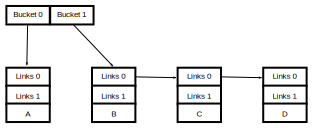
\includegraphics{datastruct/hashxu-a}}
\caption{Growing a Two-List Hash Table, State~(a)}
\label{fig:datastruct:Growing a Two-List Hash Table; State (a)}
\end{figure}

\begin{figure}
\centering
\resizebox{3in}{!}{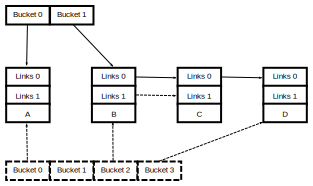
\includegraphics{datastruct/hashxu-b}}
\caption{Growing a Two-List Hash Table, State~(b)}
\label{fig:datastruct:Growing a Two-List Hash Table; State (b)}
\end{figure}

The resize operation proceeds as shown in
\crefrange{fig:datastruct:Growing a Two-List Hash Table; State (a)}
{fig:datastruct:Growing a Two-List Hash Table; State (d)},
with the initial two-bucket state shown in
\cref{fig:datastruct:Growing a Two-List Hash Table; State (a)}
and with time advancing from figure to figure.
The initial state uses the zero-index links to chain the elements into
hash buckets.
A four-bucket array is allocated, and the one-index links are used to
chain the elements into these four new hash buckets.
This results in state~(b) shown in
\cref{fig:datastruct:Growing a Two-List Hash Table; State (b)},
with readers still using the original two-bucket array.

\begin{figure}
\centering
\resizebox{3in}{!}{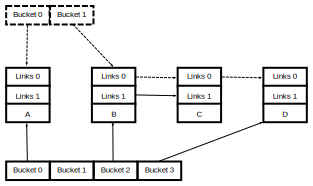
\includegraphics{datastruct/hashxu-c}}
\caption{Growing a Two-List Hash Table, State~(c)}
\label{fig:datastruct:Growing a Two-List Hash Table; State (c)}
\end{figure}

\begin{figure}
\centering
\resizebox{3in}{!}{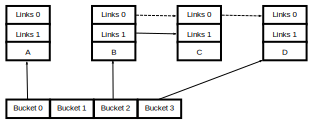
\includegraphics{datastruct/hashxu-d}}
\caption{Growing a Two-List Hash Table, State~(d)}
\label{fig:datastruct:Growing a Two-List Hash Table; State (d)}
\end{figure}

The new four-bucket array is exposed to readers and then a grace-period
operation waits for all readers, resulting in state~(c), shown in
\cref{fig:datastruct:Growing a Two-List Hash Table; State (c)}.
In this state, all readers are using the new four-bucket array,
which means that the old two-bucket array may now be freed, resulting
in state~(d), shown in
\cref{fig:datastruct:Growing a Two-List Hash Table; State (d)}.

This design leads to a relatively straightforward implementation,
which is the subject of the next section.

\subsection{Resizable Hash Table Implementation}
\label{sec:datastruct:Resizable Hash Table Implementation}

\begin{fcvref}[ln:datastruct:hash_resize:data]
Resizing is accomplished by the classic approach of inserting a level
of indirection, in this case, the \co{ht} structure shown on
\clnrefrange{ht:b}{ht:e} of
\cref{lst:datastruct:Resizable Hash-Table Data Structures}
(\path{hash_resize.c}).
The \co{hashtab} structure shown on
\clnrefrange{hashtab:b}{hashtab:e} contains only a
pointer to the current \co{ht} structure along with a spinlock that
is used to serialize concurrent attempts to resize the hash table.
If we were to use a traditional lock- or atomic-operation-based
implementation, this \co{hashtab} structure could become a severe bottleneck
from both performance and scalability viewpoints.
However, because resize operations should be relatively infrequent,
we should be able to make good use of RCU\@.

\begin{listing}
\input{CodeSamples/datastruct/hash/hash_resize@data.fcv}
\caption{Resizable Hash-Table Data Structures}
\label{lst:datastruct:Resizable Hash-Table Data Structures}
\end{listing}

The \co{ht} structure represents a specific size of the hash table,
as specified by the \co{->ht_nbuckets} field on \clnref{ht:nbuckets}.
The size is stored in the same structure containing the array of
buckets (\co{->ht_bkt[]} on
\clnref{ht:bkt}) in order to avoid mismatches between
the size and the array.
The \co{->ht_resize_cur} field on
\clnref{ht:resize_cur} is equal to $-1$ unless a resize
operation
is in progress, in which case it indicates the index of the bucket whose
elements are being inserted into the new hash table, which is referenced
by the \co{->ht_new} field on \clnref{ht:new}.
If there is no resize operation in progress, \co{->ht_new} is \co{NULL}.
Thus, a resize operation proceeds by allocating a new \co{ht} structure
and referencing it via the \co{->ht_new} pointer, then advancing
\co{->ht_resize_cur} through the old table's buckets.
When all the elements have been added to the new table, the new
table is linked into the \co{hashtab} structure's \co{->ht_cur} field.
Once all old readers have completed, the old hash table's \co{ht} structure
may be freed.

The \co{->ht_idx} field on
\clnref{ht:idx} indicates which of the two sets of
list pointers are being used by this instantiation of the hash table,
and is used to index the \co{->hte_next[]} array in the \co{ht_elem}
structure on \clnref{ht_elem:next}.

The \co{->ht_cmp()}, \co{->ht_gethash()}, and \co{->ht_getkey()} fields on
\clnrefrange{ht:cmp}{ht:getkey}
collectively define the per-element key and the hash function.
The \co{->ht_cmp()} function compares a specified key with that of
the specified element,
the \co{->ht_gethash()} calculates the specified key's hash,
and \co{->ht_getkey()} extracts the key from the enclosing data
element.

The \co{ht_lock_state} shown on \clnrefrange{hls:b}{hls:e}
is used to communicate lock state from a new \co{hashtab_lock_mod()}
to \co{hashtab_add()}, \co{hashtab_del()}, and \co{hashtab_unlock_mod()}.
This state prevents the algorithm from being redirected to the wrong
bucket during concurrent resize operations.

The \co{ht_bucket} structure is the same as before, and the
\co{ht_elem} structure differs from that of previous implementations
only in providing a two-element array of list pointer sets in place of
the prior single set of list pointers.

In a fixed-sized hash table, bucket selection is quite straightforward:
Simply transform the hash value to the corresponding bucket index.
In contrast, when resizing, updaters must also determine which of the
old and new sets of buckets to select from.
If the bucket that would be selected from the old table has already
been distributed into the new table, then the bucket should be selected
from the new table as well as from the old table.
Conversely, if the bucket that would be selected from the old table
has not yet been distributed, then the bucket should be selected from
the old table.
\end{fcvref}

\begin{listing}
\input{CodeSamples/datastruct/hash/hash_resize@get_bucket.fcv}
\caption{Resizable Hash-Table Bucket Selection}
\label{lst:datastruct:Resizable Hash-Table Bucket Selection}
\end{listing}

\begin{fcvref}[ln:datastruct:hash_resize:get_bucket]
Bucket selection is shown in
\cref{lst:datastruct:Resizable Hash-Table Bucket Selection},
which shows \co{ht_get_bucket()} on
\clnrefrange{single:b}{single:e} and \co{ht_search_bucket()} on
\clnrefrange{hsb:b}{hsb:e}.
The \co{ht_get_bucket()} function returns a reference to the bucket
corresponding to the specified key in the specified hash table, without
making any allowances for resizing.
It also stores the bucket index corresponding to the key into the location
referenced by parameter~\co{b} on
\clnref{single:gethash}, and the corresponding
hash value corresponding to the key into the location
referenced by parameter~\co{h} (if non-\co{NULL}) on \clnref{single:h}.
\Clnref{single:return} then returns a reference to the corresponding bucket.

The \co{ht_search_bucket()} function searches for the specified key
within the specified hash-table version.
\Clnref{hsb:get_curbkt} obtains a reference to the bucket corresponding
to the specified key.
The loop spanning \clnrefrange{hsb:loop:b}{hsb:loop:e} searches
that bucket, so that if \clnref{hsb:match} detects a match,
\clnref{hsb:ret_match} returns a pointer to the enclosing data element.
Otherwise, if there is no match,
\clnref{hsb:ret_NULL} returns \co{NULL} to indicate
failure.
\end{fcvref}

\QuickQuiz{
	How does the code in
	\cref{lst:datastruct:Resizable Hash-Table Bucket Selection}
	protect against the resizing process progressing past the
	selected bucket?
}\QuickQuizAnswer{
	It does not provide any such protection.
	That is instead the job of the update-side concurrency-control
	functions described next.
}\QuickQuizEnd

This implementation of \co{ht_get_bucket()} and \co{ht_search_bucket()}
permits lookups and modifications to run concurrently with a resize
operation.

\begin{listing}
\input{CodeSamples/datastruct/hash/hash_resize@lock_unlock_mod.fcv}
\caption{Resizable Hash-Table Update-Side Concurrency Control}
\label{lst:datastruct:Resizable Hash-Table Update-Side Concurrency Control}
\end{listing}

Read-side concurrency control is provided by RCU as was shown in
\cref{lst:datastruct:RCU-Protected Hash-Table Read-Side Concurrency Control},
but the update-side concurrency\-/control functions
\co{hashtab_lock_mod()} and \co{hashtab_unlock_mod()}
must now deal with the possibility of a
concurrent resize operation as shown in
\cref{lst:datastruct:Resizable Hash-Table Update-Side Concurrency Control}.

\begin{fcvref}[ln:datastruct:hash_resize:lock_unlock_mod:l]
The \co{hashtab_lock_mod()} spans
\clnrefrange{b}{e} in the listing.
\Clnref{rcu_lock} enters an RCU read-side critical section to prevent
the data structures from being freed during the traversal,
\clnref{refhashtbl} acquires a reference to the current hash table, and then
\clnref{refbucket} obtains a reference to the bucket in this hash table
corresponding to the key.
\Clnref{acq_bucket} acquires that bucket's lock, which will prevent any concurrent
resizing operation from distributing that bucket, though of course it
will have no effect if that bucket has already been distributed.
\Clnrefrange{lsp0b}{lsp0e} store the bucket pointer and
pointer-set index into their respective fields in the
\co{ht_lock_state} structure, which communicates the information to
\co{hashtab_add()}, \co{hashtab_del()}, and \co{hashtab_unlock_mod()}.
\Clnref{ifresized} then checks to see if a concurrent resize
operation has already distributed this bucket across the new hash table,
and if not, \clnref{lsp1_1} indicates that there is no
already-resized hash bucket and
\clnref{fastret1} returns with the selected hash bucket's
lock held (thus preventing a concurrent resize operation from distributing
this bucket) and also within an RCU read-side critical section.
\IX{Deadlock} is avoided because the old table's locks are always acquired
before those of the new table, and because the use of RCU prevents more
than two versions from existing at a given time, thus preventing a
deadlock cycle.

Otherwise, a concurrent resize operation has already distributed this
bucket, so \clnref{new_hashtbl} proceeds to the new hash table,
\clnref{get_newbkt} selects the bucket corresponding to the key,
and \clnref{acq_newbkt} acquires the bucket's lock.
\Clnrefrange{lsp1b}{lsp1e} store the new-table bucket pointer and
pointer-set index into their respective fields in the
\co{ht_lock_state} structure, which again communicates this information to
\co{hashtab_add()}, \co{hashtab_del()}, and \co{hashtab_unlock_mod()}.
Because this bucket has already been resized and because
\co{hashtab_add()} and \co{hashtab_del()} affect both the old and the
new \co{ht_bucket} structures, two locks are held, one on each of the
two buckets.
Additionally, both elements of each array in \co{ht_lock_state} structure
are used, with the \co{[0]} element pertaining to the old \co{ht_bucket}
structure and the \co{[1]} element pertaining to the new structure.
Once again, \co{hashtab_lock_mod()} exits within an RCU read-side critical
section.
\end{fcvref}

\begin{fcvref}[ln:datastruct:hash_resize:lock_unlock_mod:ul]
The \co{hashtab_unlock_mod()} function releases the lock(s) acquired by
\co{hashtab_lock_mod()}.
\Clnref{relbkt0} releases the lock on the old \co{ht_bucket} structure.
In the unlikely event that \clnref{ifbkt1} determines that a resize
operation is in progress, \clnref{relbkt1} releases the lock on the
new \co{ht_bucket} structure.
Either way, \clnref{rcu_unlock} exits the RCU read-side critical
section.
\end{fcvref}

\QuickQuiz{
	Suppose that one thread is inserting an element into the
	hash table during a resize operation.
	What prevents this insertion from being lost due to a subsequent
	resize operation completing before the insertion does?
}\QuickQuizAnswer{
	The second resize operation will not be able to move beyond
	the bucket into which the insertion is taking place due to
	the insertion holding the lock(s) on one or both of the hash
	buckets in the hash tables.
	Furthermore, the insertion operation takes place within an
	RCU read-side critical section.
	As we will see when we examine the \co{hashtab_resize()}
	function, this allows each resize operation to use
	\co{synchronize_rcu()} invocations to wait for the insertion's
	read-side critical section to complete.
	These \co{synchronize_rcu()} invocations prevent pre-existing
	insertions operation from outliving the resize operation.
}\QuickQuizEnd

\begin{listing}
\input{CodeSamples/datastruct/hash/hash_resize@access.fcv}
\caption{Resizable Hash-Table Access Functions}
\label{lst:datastruct:Resizable Hash-Table Access Functions}
\end{listing}

Now that we have bucket selection and concurrency control in place,
we are ready to search and update our resizable hash table.
The \co{hashtab_lookup()}, \co{hashtab_add()}, and \co{hashtab_del()}
functions are shown in
\cref{lst:datastruct:Resizable Hash-Table Access Functions}.

\begin{fcvref}[ln:datastruct:hash_resize:access:lkp]
The \co{hashtab_lookup()} function on
\clnrefrange{b}{e} of the listing does
hash lookups.
\Clnref{get_curtbl} fetches the current hash table and
\clnref{get_curbkt} searches the bucket corresponding to the
specified key.
\Clnref{ret} returns a pointer to the searched-for element
or \co{NULL} when the search fails.
The caller must be within an RCU read-side critical section.
\end{fcvref}

\QuickQuiz{
	The \co{hashtab_lookup()} function in
	\cref{lst:datastruct:Resizable Hash-Table Access Functions}
	ignores concurrent resize operations.
	Doesn't this mean that readers might miss an element that was
	previously added during a resize operation?
}\QuickQuizAnswer{
	No.
	As we will see soon,
	the \co{hashtab_add()} and \co{hashtab_del()} functions
	keep the old hash table up-to-date while a resize operation
	is in progress.
}\QuickQuizEnd

\begin{fcvref}[ln:datastruct:hash_resize:access:add]
The \co{hashtab_add()} function on \clnrefrange{b}{e} of the listing adds
new data elements to the hash table.
\Clnref{htbp} picks up the current \co{ht_bucket} structure into which the
new element is to be added, and \clnref{i} picks up the index of
the pointer pair.
\Clnref{add} adds the new element to the current hash bucket.
If \clnref{ifnew} determines that this bucket has been distributed
to a new version of the hash table, then \clnref{addnew} also adds the
new element to the corresponding new bucket.
The caller is required to handle concurrency, for example, by invoking
\co{hashtab_lock_mod()} before the call to \co{hashtab_add()} and invoking
\co{hashtab_unlock_mod()} afterwards.
\end{fcvref}

\begin{fcvref}[ln:datastruct:hash_resize:access:del]
The \co{hashtab_del()} function on
\clnrefrange{b}{e} of the listing removes
an existing element from the hash table.
\Clnref{i} picks up the index of the pointer pair
and \clnref{del} removes the specified element from the current table.
If \clnref{ifnew} determines that this bucket has been distributed
to a new version of the hash table, then \clnref{delnew} also removes
the specified element from the corresponding new bucket.
As with \co{hashtab_add()}, the caller is responsible for concurrency
control and this concurrency control suffices for synchronizing with
a concurrent resize operation.
\end{fcvref}

\QuickQuiz{
	The \co{hashtab_add()} and \co{hashtab_del()} functions in
	\cref{lst:datastruct:Resizable Hash-Table Access Functions}
	can update two hash buckets while a resize operation is progressing.
	This might cause poor performance if the frequency of resize operation
	is not negligible.
	Isn't it possible to reduce the cost of updates in such cases?
}\QuickQuizAnswer{
	Yes, at least assuming that a slight increase in the cost of
	\co{hashtab_lookup()} is acceptable.
	One approach is shown in
	\cref{lst:datastruct:Resizable Hash-Table Access Functions (Fewer Updates),%
	lst:datastruct:Resizable Hash-Table Update-Side Locking Function (Fewer Updates)}
	(\path{hash_resize_s.c}).

\begin{listing}
\input{CodeSamples/datastruct/hash/hash_resize_s@access.fcv}
\caption{Resizable Hash-Table Access Functions (Fewer Updates)}
\label{lst:datastruct:Resizable Hash-Table Access Functions (Fewer Updates)}
\end{listing}

\begin{listing}
\input{CodeSamples/datastruct/hash/hash_resize_s@lock_mod.fcv}
\caption{Resizable Hash-Table Update-Side Locking Function (Fewer Updates)}
\label{lst:datastruct:Resizable Hash-Table Update-Side Locking Function (Fewer Updates)}
\end{listing}

	This version of \co{hashtab_add()} adds an element to
	either the old bucket if it is not resized yet, or to the new
	bucket if it has been resized, and \co{hashtab_del()} removes
	the specified element from any buckets into which it has been inserted.
	The \co{hashtab_lookup()} function searches the new bucket
	if the search of the old bucket fails, which has the disadvantage
	of adding overhead to the lookup fastpath.
	The alternative \co{hashtab_lock_mod()} returns the locking
	state of the new bucket in \co{->hbp[0]} and \co{->hls_idx[0]}
	if resize operation is in progress, instead of the perhaps
	more natural choice of \co{->hbp[1]} and \co{->hls_idx[1]}.
	However, this less-natural choice has the advantage of simplifying
	\co{hashtab_add()}.

	Further analysis of the code is an exercise for the reader.
}\QuickQuizEnd

\begin{listing*}
\input{CodeSamples/datastruct/hash/hash_resize@resize.fcv}
\caption{Resizable Hash-Table Resizing}
\label{lst:datastruct:Resizable Hash-Table Resizing}
\end{listing*}

\begin{fcvref}[ln:datastruct:hash_resize:resize]
The actual resizing itself is carried out by \co{hashtab_resize()}, shown in
\cref{lst:datastruct:Resizable Hash-Table Resizing} on
\cpageref{lst:datastruct:Resizable Hash-Table Resizing}.
\Clnref{trylock} conditionally acquires the top-level \co{->ht_lock}, and if
this acquisition fails, \clnref{ret_busy} returns \co{-EBUSY} to indicate that
a resize is already in progress.
Otherwise, \clnref{get_curtbl} picks up a reference to the current hash table,
and \clnrefrange{alloc:b}{alloc:e} allocate a new hash table of the desired size.
If a new set of hash/key functions have been specified, these are
used for the new table, otherwise those of the old table are preserved.
If \clnref{chk_nomem} detects memory-allocation failure,
\clnref{rel_nomem} releases \co{->ht_lock}
and \clnref{ret_nomem} returns a failure indication.

\Clnref{get_curidx} picks up the current table's index and
\clnref{put_curidx} stores its inverse to
the new hash table, thus ensuring that the two hash tables avoid overwriting
each other's linked lists.
\Clnref{set_newtbl} then starts the bucket-distribution process by
installing a reference to the new table into the \co{->ht_new} field of
the old table.
\Clnref{sync_rcu} ensures that all readers who are not aware of the
new table complete before the resize operation continues.

Each pass through the loop spanning \clnrefrange{loop:b}{loop:e} distributes the contents
of one of the old hash table's buckets into the new hash table.
\Clnref{get_oldcur} picks up a reference to the old table's current bucket
and \clnref{acq_oldcur} acquires that bucket's spinlock.
\end{fcvref}

\QuickQuiz{
	\begin{fcvref}[ln:datastruct:hash_resize:resize]
	In the \co{hashtab_resize()} function in
	\cref{lst:datastruct:Resizable Hash-Table Resizing},
	what guarantees that the update to \co{->ht_new} on \clnref{set_newtbl}
	will be seen as happening before the update to \co{->ht_resize_cur}
	on \clnref{update_resize} from the perspective of
	\co{hashtab_add()} and \co{hashtab_del()}?
	In other words, what prevents \co{hashtab_add()}
	and \co{hashtab_del()} from dereferencing
	a \co{NULL} pointer loaded from \co{->ht_new}?
	\end{fcvref}
}\QuickQuizAnswer{
	\begin{fcvref}[ln:datastruct:hash_resize:resize]
	The \co{synchronize_rcu()} on \clnref{sync_rcu} of
	\cref{lst:datastruct:Resizable Hash-Table Resizing}
	ensures that all pre-existing RCU readers have completed between
	the time that we install the new hash-table reference on
	\clnref{set_newtbl} and the time that we update \co{->ht_resize_cur} on
	\clnref{update_resize}.
	This means that any reader that sees a non-negative value
	of \co{->ht_resize_cur} cannot have started before the
	assignment to \co{->ht_new}, and thus must be able to see
	the reference to the new hash table.

	And this is why the update-side \co{hashtab_add()} and
	\co{hashtab_del()} functions must be enclosed
	in RCU read-side critical sections, courtesy of
	\co{hashtab_lock_mod()} and \co{hashtab_unlock_mod()} in
	\cref{lst:datastruct:Resizable Hash-Table Update-Side Concurrency Control}.
	\end{fcvref}
}\QuickQuizEnd

\begin{fcvref}[ln:datastruct:hash_resize:resize]
Each pass through the loop spanning
\clnrefrange{loop_list:b}{loop_list:e} adds one data element
from the current old-table bucket to the corresponding new-table bucket,
holding the new-table bucket's lock during the add operation.
\Clnref{update_resize} updates
\co{->ht_resize_cur} to indicate that this bucket has been distributed.
Finally, \clnref{rel_oldcur} releases the old-table bucket lock.

Execution reaches \clnref{rcu_assign} once all old-table buckets have been distributed
across the new table.
\Clnref{rcu_assign} installs the newly created table as the current one, and
\clnref{sync_rcu_2} waits for all old readers (who might still be referencing
the old table) to complete.
Then \clnref{rel_master} releases the resize-serialization lock,
\clnref{free} frees
the old hash table, and finally \clnref{ret_success} returns success.
\end{fcvref}

\QuickQuiz{
	\begin{fcvref}[ln:datastruct:hash_resize:resize]
	Why is there a \co{WRITE_ONCE()} on \clnref{update_resize}
	in \cref{lst:datastruct:Resizable Hash-Table Resizing}?
	\end{fcvref}
}\QuickQuizAnswer{
	\begin{fcvref}[ln:datastruct:hash_resize:lock_unlock_mod]
	Together with the \co{READ_ONCE()}
	on \clnref{l:ifresized} in \co{hashtab_lock_mod()}
	of \cref{lst:datastruct:Resizable Hash-Table Update-Side Concurrency Control},
	it tells the compiler that the non-initialization accesses
	to \co{->ht_resize_cur} must remain because reads
	from \co{->ht_resize_cur} really can race with writes,
	just not in a way to change the ``if'' conditions.
	\end{fcvref}
}\QuickQuizEnd

\subsection{Resizable Hash Table Discussion}
\label{sec:datastruct:Resizable Hash Table Discussion}

\begin{figure}
\centering
\resizebox{2.7in}{!}{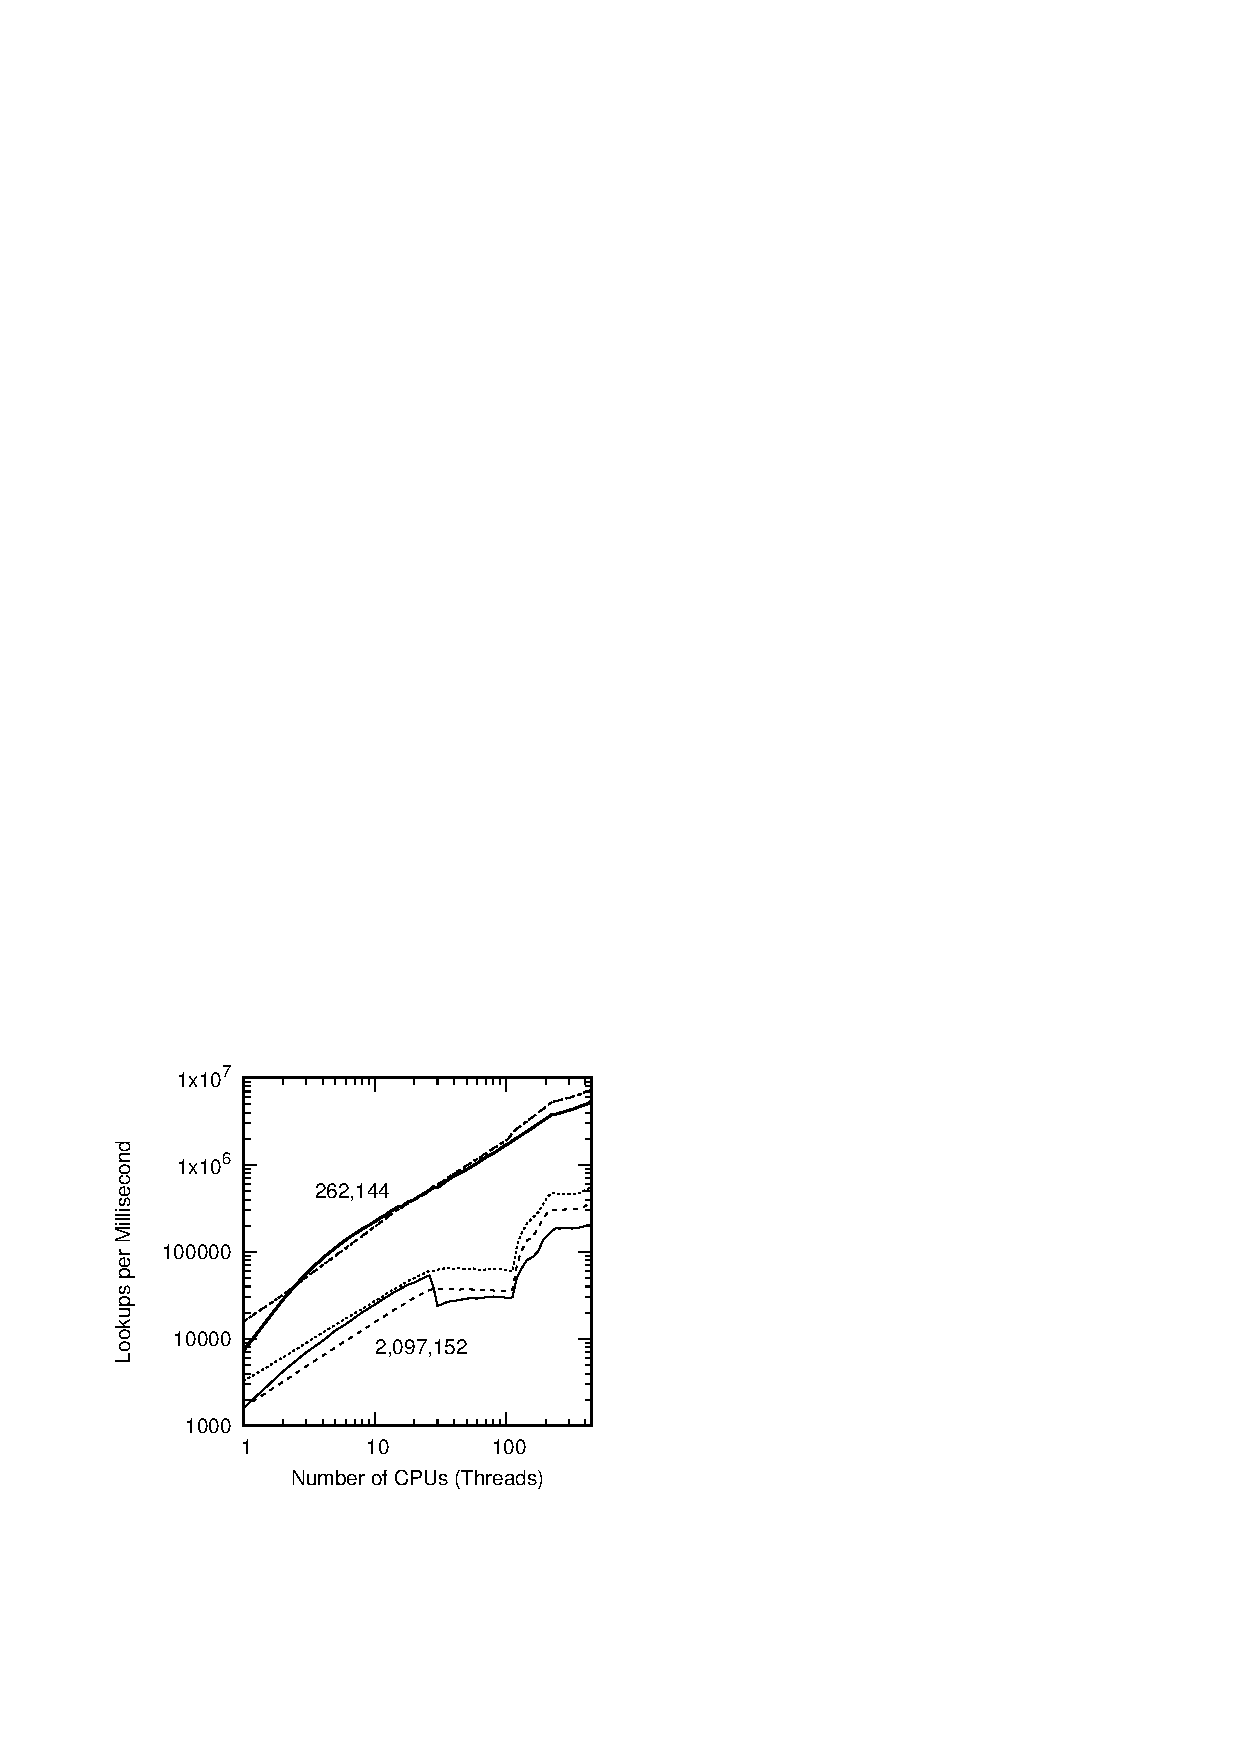
\includegraphics{CodeSamples/datastruct/hash/data/hps.resize.2020.09.05a/perftestresize}}
\caption{Overhead of Resizing Hash Tables Between 262,144 and 524,288 Buckets vs.\@ Total Number of Elements}
\label{fig:datastruct:Overhead of Resizing Hash Tables Between 262;144 and 524;288 Buckets vs. Total Number of Elements}
\end{figure}

\Cref{fig:datastruct:Overhead of Resizing Hash Tables Between 262;144 and 524;288 Buckets vs. Total Number of Elements}
compares resizing hash tables to their fixed-sized counterparts
for 262,144 and 2,097,152 elements in the hash table.
The figure shows three traces for each element count, one
for a fixed-size 262,144-bucket hash table, another for a
fixed-size 524,288-bucket hash table, and a third for a resizable
hash table that shifts back and forth between 262,144 and 524,288
buckets, with a one-millisecond pause between each resize operation.

The uppermost three traces are for the 262,144-element hash table.\footnote{
	You see only two traces?
	The dashed one is composed of two traces that differ
	only slightly, hence the irregular-looking dash pattern.}
The dashed trace corresponds to the two fixed-size hash tables,
and the solid trace to the resizable hash table.
In this case, the short hash chains cause normal lookup overhead
to be so low that the overhead of resizing dominates over most
of the range.
In particular, the entire hash table fits into L3 cache.
% Nevertheless, the larger fixed-size hash table has a significant
% performance advantage, so that resizing can be quite beneficial,
% at least given sufficient time between resizing operations: One
% millisecond is clearly too short a time.

The lower three traces are for the 2,097,152-element hash table.
The upper dashed trace corresponds to the 262,144-bucket fixed-size
hash table, the solid trace in the middle for low CPU counts and at
the bottom for high CPU counts to the resizable hash table,
and the other trace to the 524,288-bucket fixed-size hash table.
The fact that there are now an average of eight elements per bucket
can only be expected to produce a sharp decrease in performance,
as in fact is shown in the graph.
But worse yet, the hash-table elements occupy 128\,MB, which overflows
each socket's 39\,MB L3 cache, with performance consequences analogous
to those described in \cref{sec:cpu:Costs of Operations}.
The resulting cache overflow means that the memory system is involved
even for a read-only benchmark, and as you can see from the sublinear
portions of the lower three traces, the memory system can be a serious
bottleneck.

\QuickQuiz{
	How much of the difference in performance between the large and
	small hash tables shown in
	\cref{fig:datastruct:Overhead of Resizing Hash Tables Between 262;144 and 524;288 Buckets vs. Total Number of Elements}
	was due to long hash chains and how much was due to
	memory-system bottlenecks?
}\QuickQuizAnswer{
	The easy way to answer this question is to do another run with
	2,097,152 elements, but this time also with 2,097,152 buckets,
	thus bringing the average number of elements per bucket back down
	to unity.

\begin{figure}
\centering
\resizebox{2.7in}{!}{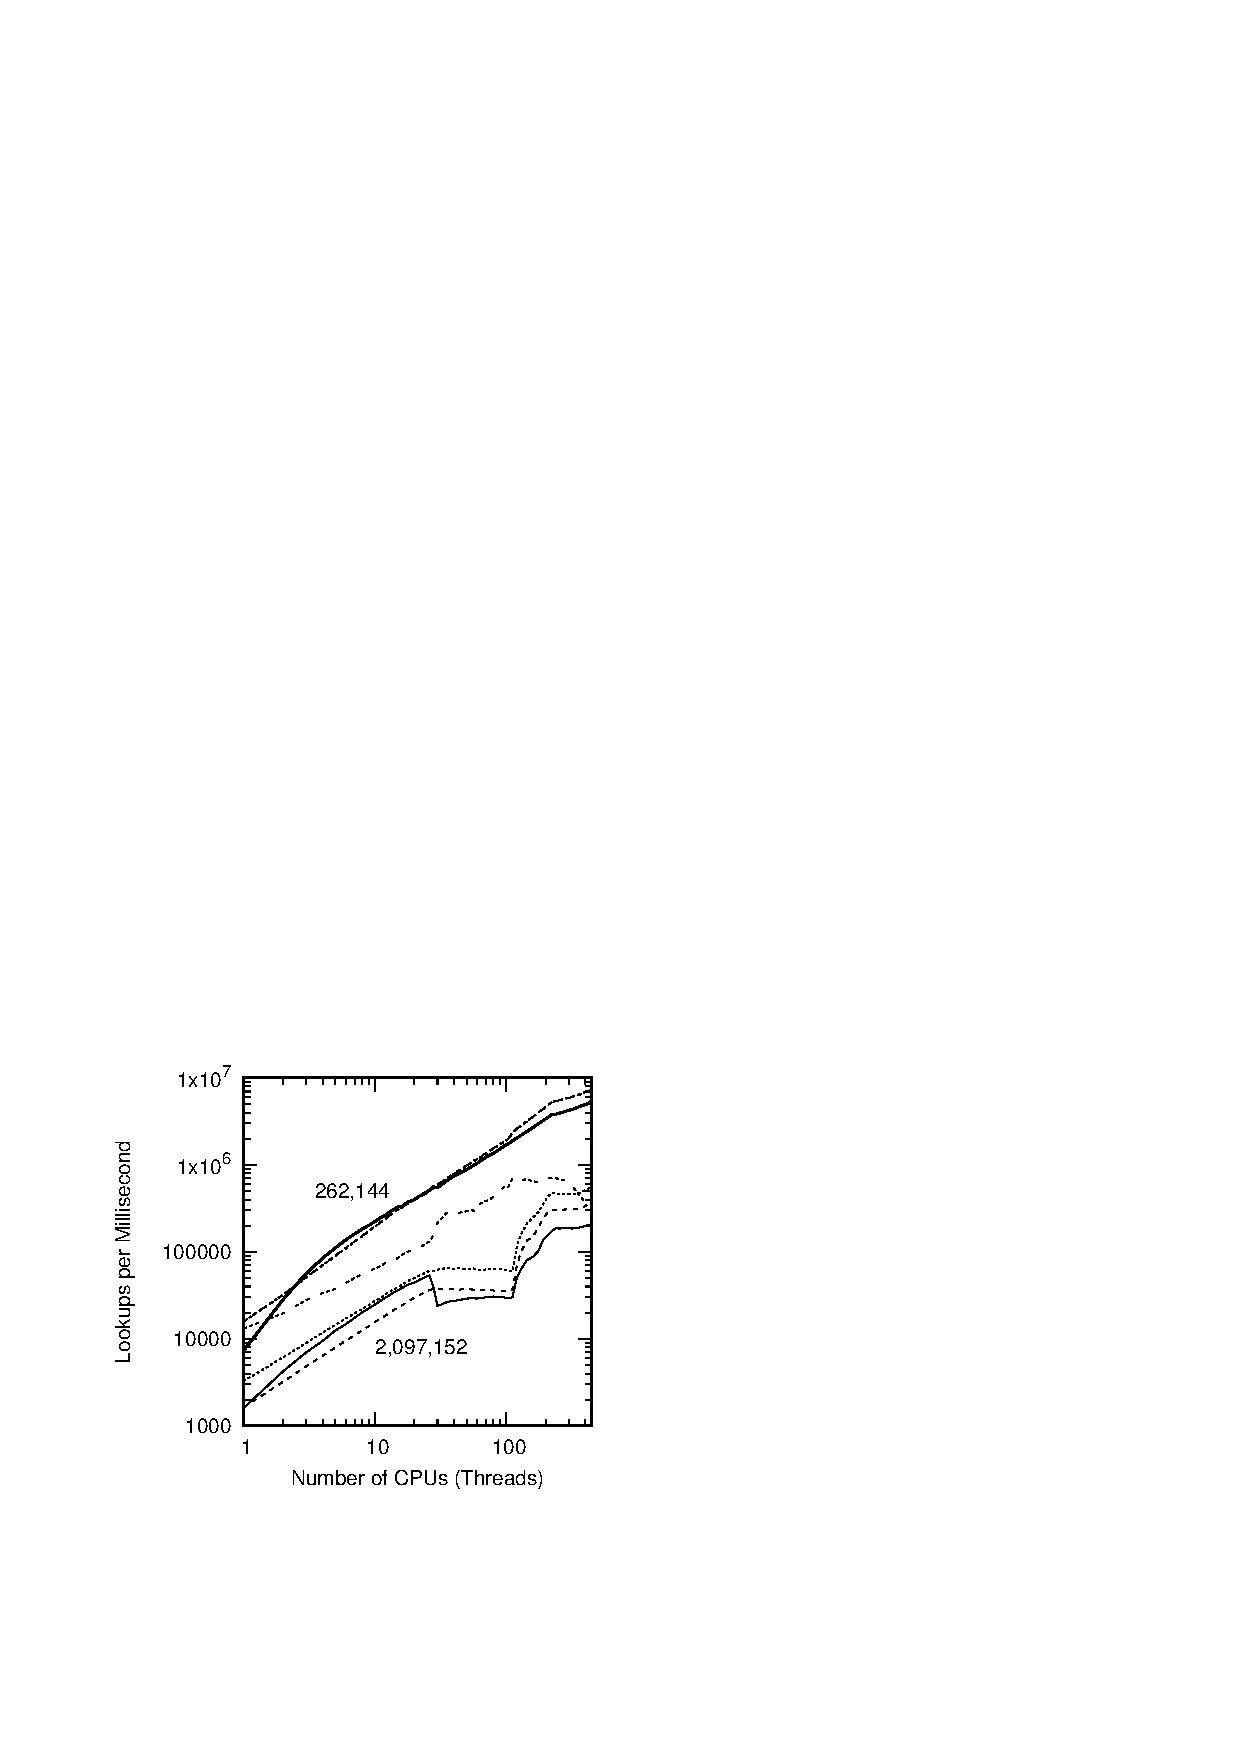
\includegraphics{CodeSamples/datastruct/hash/data/hps.resize.2020.09.27a/perftestresizebig}}
\caption{Effect of Memory-System Bottlenecks on Hash Tables}
\label{fig:datastruct:Effect of Memory-System Bottlenecks on Hash Tables}
\end{figure}

	The results are shown by the triple-dashed new trace in
	the middle of
	\cref{fig:datastruct:Effect of Memory-System Bottlenecks on Hash Tables}.
	The other six traces are identical to their counterparts in
	\cref{fig:datastruct:Overhead of Resizing Hash Tables Between 262;144 and 524;288 Buckets vs. Total Number of Elements}
	on \cpageref{fig:datastruct:Overhead of Resizing Hash Tables Between 262;144 and 524;288 Buckets vs. Total Number of Elements}.
	The gap between this new trace and the lower set of three
	traces is a rough measure of how much of the difference in
	performance was due to hash-chain length, and the gap between
	the new trace and the upper set of three traces is a rough measure
	of how much of that difference was due to memory-system bottlenecks.
	The new trace starts out slightly below its 262,144-element
	counterpart at a single CPU, showing that cache capacity is
	degrading performance slightly even on that single CPU\@.\footnote{
		Yes, as far as hardware architects are concerned,
		caches are part of the memory system.}
	This is to be expected, given that unlike its smaller counterpart,
	the 2,097,152-bucket hash table does not fit into the L3 cache.
	This new trace rises just past 28~CPUs, which is also to be
	expected.
	This rise is due to the fact that the 29\textsuperscript{th}
	CPU is on another socket, which brings with it an additional
	39\,MB of cache as well as additional memory bandwidth.

	But the large hash table's advantage over that of the hash table
	with 524,288~buckets (but still 2,097,152 elements) decreases
	with additional CPUs, which is consistent with the bottleneck
	residing in the memory system.
	Above about 400~CPUs, the 2,097,152-bucket hash table is
	actually outperformed slightly by the 524,288-bucket hash
	table.
	This should not be a surprise because the memory system is
	the bottleneck and the larger number of buckets increases this
	workload's memory footprint.

	The alert reader will have noted the word ``rough'' above
	and might be interested in a more detailed analysis.
	Such readers are invited to run similar benchmarks, using
	whatever performance counters or hardware-analysis tools
	they might have available.
	This can be a long and complex journey, but those brave enough
	to embark on it will be rewarded with detailed knowledge of
	hardware performance and its effect on software.
}\QuickQuizEnd

Referring to the last column of
\cref{tab:cpu:CPU 0 View of Synchronization Mechanisms on 8-Socket System With Intel Xeon Platinum 8176 CPUs at 2.10GHz},
we recall that the first 28~CPUs are in the first socket, on a
one-CPU-per-core basis, which explains the sharp decrease in performance
of the resizable hash table beyond 28~CPUs.
Sharp though this decrease is, please recall that it is due to constant
resizing back and forth.
It would clearly be better to resize once to 524,288 buckets,
or, even better, do a single eight-fold resize to 2,097,152 elements,
thus dropping the average number of elements per bucket down to the
level enjoyed by the runs producing the upper three traces.

The key point from this data is that the RCU-protected resizable hash
table performs and scales almost as well as does its fixed-size counterpart.
The performance during an actual resize operation of course suffers
somewhat due to the cache misses causes by the updates to each element's
pointers, and this effect is most pronounced when the memory system
becomes a bottleneck.
This indicates that hash tables should be resized by substantial amounts,
and that hysteresis should be applied to prevent performance degradation
due to too-frequent resize operations.
In memory-rich environments, hash-table sizes should furthermore
be increased much more aggressively than they are decreased.

Another key point is that although the \co{hashtab} structure is
non-partitionable, it is also read-mostly, which suggests the use
of RCU\@.
Given that the performance and scalability of this resizable hash table is
very nearly that of RCU-protected fixed-sized hash tables, we must
conclude that this approach was quite successful.

Finally, it is important to note that insertions, deletions, and
lookups can proceed concurrently with a resize operation.
This concurrency is
critically important when resizing large hash tables, especially
for applications that must meet severe response-time constraints.

Of course, the \co{ht_elem} structure's
pair of pointer sets does impose some memory overhead,
which is taken up in the next section.

\subsection{Other Resizable Hash Tables}
\label{sec:datastruct:Other Resizable Hash Tables}

One shortcoming of the resizable hash table described earlier in this
section is memory consumption.
Each data element has two pairs of linked-list pointers rather than just
one.
Is it possible to create an RCU-protected resizable hash table that
makes do with just one pair?

It turns out that the answer is ``yes''.
Josh Triplett et al.~\cite{Triplett:2011:RPHash}
produced a \emph{relativistic hash table} that incrementally
splits and combines corresponding hash chains so that readers always
see valid hash chains at all points during the resizing operation.
This incremental splitting and combining relies on the fact that it
is harmless for a reader to see a data element that should be in some
other hash chain:
When this happens, the reader will simply ignore the extraneous data
element due to key mismatches.

\begin{figure}
\centering
\resizebox{3in}{!}{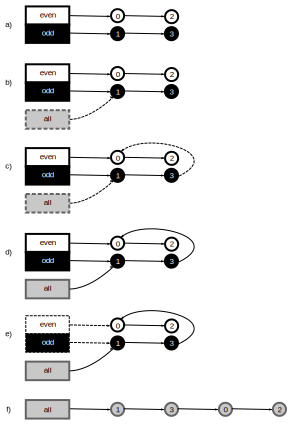
\includegraphics{datastruct/zipperhashshrink}}
\caption{Shrinking a Relativistic Hash Table}
\label{fig:datastruct:Shrinking a Relativistic Hash Table}
\end{figure}

The process of shrinking a relativistic hash table by a factor of two
is shown in
\cref{fig:datastruct:Shrinking a Relativistic Hash Table},
in this case shrinking a two-bucket hash table into a one-bucket
hash table, otherwise known as a linear list.
This process works by coalescing pairs of buckets in the old larger hash
table into single buckets in the new smaller hash table.
For this process to work correctly, we clearly need to constrain the hash
functions for the two tables.
One such constraint is to use the same underlying hash function for
both tables, but to throw out the low-order bit when shrinking from
large to small.
For example, the old two-bucket hash table would
use the two top bits of the value, while the new one-bucket hash table
could use the top bit of the value.
In this way, a given pair of adjacent even and odd buckets in the old
large hash table can be coalesced into a single bucket in the new small
hash table, while still having a single hash value cover all of the
elements in that single bucket.

The initial state is shown at the top of the figure, with time advancing
from top to bottom, starting with initial state~(a).
The shrinking process begins by allocating the new smaller array of
buckets, and having each bucket of this new smaller array reference
the first element of one of the buckets of the corresponding pair in
the old large hash table, resulting in state~(b).

Then the two hash chains are linked together, resulting in state~(c).
In this state, readers looking up an even-numbered element see no change,
and readers looking up elements~1 and~3 likewise see no change.
However, readers looking up some other odd number will also traverse
elements~0 and~2.
This is harmless because any odd number will compare not-equal to these
two elements.
There is some performance loss, but on the other hand, this is exactly
the same performance loss that will be experienced once the new small
hash table is fully in place.

Next, the new small hash table is made accessible to readers, resulting
in state~(d).
Note that older readers might still be traversing the old large hash
table, so in this state both hash tables are in use.

The next step is to wait for all pre-existing readers to complete,
resulting in state~(e).
In this state, all readers are using the new small hash table, so that
the old large hash table's buckets may be freed, resulting in the final
state~(f).

\begin{figure}
\centering
\resizebox{3in}{!}{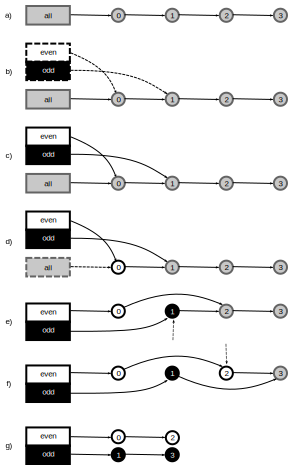
\includegraphics{datastruct/zipperhashgrow}}
\caption{Growing a Relativistic Hash Table}
\label{fig:datastruct:Growing a Relativistic Hash Table}
\end{figure}

Growing a relativistic hash table reverses the shrinking process,
but requires more grace-period steps, as shown in
\cref{fig:datastruct:Growing a Relativistic Hash Table}.
The initial state~(a) is at the top of this figure, with time advancing
from top to bottom.

We start by allocating the new large two-bucket hash table, resulting
in state~(b).
Note that each of these new buckets references the first element destined
for that bucket.
These new buckets are published to readers, resulting in state~(c).
After a grace-period operation, all readers are using the new large
hash table, resulting in state~(d).
In this state, only those readers traversing the even-values hash bucket
traverse element~0, which is therefore now colored white.

At this point, the old small hash buckets may be freed, although many
implementations use these old buckets to track progress ``unzipping''
the list of items into their respective new buckets.
The last even-numbered element in the first consecutive run of such
elements now has its pointer-to-next updated to reference the following
even-numbered element.
After a subsequent grace-period operation, the result is state~(e).
The vertical arrow indicates the next element to be unzipped, and
element~1 is now colored black to indicate that only those readers traversing
the odd-values hash bucket may reach it.

Next, the last odd-numbered element in the first consecutive run of such
elements now has its pointer-to-next updated to reference the following
odd-numbered element.
After a subsequent grace-period operation, the result is state~(f).
A final unzipping operation (including a grace-period operation)
results in the final state~(g).

In short, the relativistic hash table reduces the number of per-element
list pointers at the expense of additional grace periods incurred during
resizing.
These additional grace periods are usually not a problem because
insertions, deletions, and lookups may proceed concurrently with
a resize operation.

However, when a hash table is growing quickly, the large numbers of
grace periods might delay the beginning of the next resize operation.
One way to reduce the number of grace periods is to unzip all the
buckets concurrently, so that the number of grace periods will be
limited by the largest number of elements in a single bucket instead
of by the total number of elements in the hash table.
Another approach, also by Josh Triplett, is to maintain a separate
pointer to the element currently being moved from the old bucket to
the new bucket.
Readers then check the old bucket, the separate pointer, and the new
bucket in order.
This requires read-side memory ordering, which slows readers, but
it greatly reduces the required number of resize-time grace periods.
This approach is used within the Linux kernel.

It turns out that it is possible to reduce the per-element memory overhead
from a pair of pointers to a single pointer, while still retaining
$\O{1}$ deletions.
This is accomplished by augmenting split-order
list~\cite{OriShalev2006SplitOrderListHash}
with RCU
protection~\cite{MathieuDesnoyers2009URCU,PaulMcKenney2013LWNURCUhash}.
The data elements in the hash table are arranged into a single
sorted linked list, with each hash bucket referencing the first element
in that bucket.
Elements are deleted by setting low-order bits in their pointer-to-next
fields, and these elements are removed from the list by later traversals
that encounter them.

This RCU-protected split-order list is complex, but offers lock-free
progress guarantees for all insertion, deletion, and lookup operations.
Such guarantees can be important in real-time applications.
However, one downside is that the keys must be bit-reversed during
lookup, which slows down readers.
But for those for whom this slowdown is not a problem, an
implementation is available from recent versions of the userspace RCU
library~\cite{MathieuDesnoyers2009URCU}.

\section{Other Data Structures}
\label{sec:datastruct:Other Data Structures}
%
\epigraph{All life is an experiment.
	  The more experiments you make the better.}
	 {Ralph Waldo Emerson}

The preceding sections have focused on data structures that enhance
concurrency due to partitionability
(\cref{sec:datastruct:Partitionable Data Structures}),
efficient handling of read-mostly access patterns
(\cref{sec:datastruct:Read-Mostly Data Structures}),
or application of read-mostly techniques to avoid
non-partitionability
(\cref{sec:datastruct:Non-Partitionable Data Structures}).
This section gives a brief review of other data structures.

One of the hash table's greatest advantages for parallel use is that it
is fully partitionable, at least while not being resized.
One way of preserving the partitionability and the size independence is
to use a radix tree, which is also called a trie.
Tries partition the search key, using each successive key partition
to traverse the next level of the trie.
As such, a trie can be thought of as a set of nested hash tables,
thus providing the required partitionability.
One disadvantage of tries is that a sparse key space can result in
inefficient use of memory.
There are a number of compression techniques that may be used to
work around this disadvantage, including hashing the key value to
a smaller keyspace before the
traversal~\cite{RobertOlsson2007Trash}.
Radix trees are heavily used in practice, including in the Linux
kernel~\cite{NickPiggin2006radixtree}.

One important special case of both a hash table and a trie is what is
perhaps the oldest of data structures, the array and its multi-dimensional
counterpart, the matrix.
The fully partitionable nature of matrices is exploited heavily in
concurrent numerical algorithms.

Self-balancing trees are heavily used in sequential code, with
AVL trees and red-black trees being perhaps the most well-known
examples~\cite{ThomasHCorman2001Algorithms}.
Early attempts to parallelize AVL trees were complex and not necessarily
all that efficient~\cite{Ellis80},
however, more recent work on red-black trees provides better
performance and scalability by using RCU for readers and hashed arrays
of locks\footnote{
	In the guise of swissTM~\cite{AleksandarDragovejic2011STMnotToy},
	which is a variant of software transactional memory in which
	the developer flags non-shared accesses.}
to protect reads and updates,
respectively~\cite{PhilHoward2011RCUTMRBTree,PhilipWHoward2013RCUrbtree}.
It turns out that red-black trees rebalance aggressively, which works
well for sequential programs, but not necessarily so well for parallel
use.
Recent work has therefore made use of RCU-protected ``bonsai trees''
that rebalance less aggressively~\cite{AustinClements2012RCULinux:mmapsem},
trading off optimal tree depth to gain more efficient concurrent updates.

Concurrent skip lists lend themselves well to RCU readers, and in fact
represents an early academic use of a technique resembling
RCU~\cite{Pugh90}.
% @@@ Reference skiplist chapter once added.

Concurrent double-ended queues were discussed in
\cref{sec:SMPdesign:Double-Ended Queue},
and concurrent stacks and queues have a long history~\cite{Treiber86},
though not normally the most impressive performance or scalability.
They are nevertheless a common feature of concurrent
libraries~\cite{PaulMcKenney2013LWNURCUqueuestack}.
Researchers have recently proposed relaxing the ordering constraints
of stacks and queues~\cite{Shavit:2011:DSM:1897852.1897873},
with some work indicating that relaxed-ordered queues actually have
better ordering properties than do strict FIFO
queues~\cite{AndreasHaas2012FIFOisnt,ChristophMKirsch2012FIFOisntTR,AndreasHaas2013CFRelaxedQueues}.

It seems likely that continued work with concurrent data structures will
produce novel algorithms with surprising properties.

\section{Summary}
\label{sec:datastruct:Summary}
%
\epigraph{There's only one thing more painful than learning from
	  experience, and that is not learning from experience.}
	 {Archibald MacLeish}

This chapter has focused primarily on hash tables, including resizable
hash tables, which are not fully partitionable.
\Cref{sec:datastruct:Other Data Structures} gave a quick
overview of a few non-hash-table data structures.
Nevertheless, this exposition of hash tables is an excellent introduction
to the many issues surrounding high-performance scalable data access,
including:

\begin{enumerate}
\item	Fully partitioned data structures work well on small systems,
	for example, single-socket systems.
\item	Larger systems require locality of reference as well as
	full partitioning.
\item	Read-mostly techniques, such as hazard pointers and RCU,
	provide good locality of reference for read-mostly workloads,
	and thus provide excellent performance and scalability even
	on larger systems.
\item	Read-mostly techniques also work well on some types of
	non-partitionable data structures, such as resizable hash tables.
\item	Large data structures can overflow CPU caches, reducing performance
	and scalability.
\item	Additional performance and scalability can be obtained by
	specializing the data structure to a specific workload,
	for example, by replacing a general key with a 32-bit integer.
\item	Although requirements for portability and for extreme performance
	often conflict, there are some data-structure-layout techniques
	that can strike a good balance between these two sets of
	requirements.
\end{enumerate}

That said, performance and scalability are of little use without reliability,
so the next chapter covers validation.

\QuickQuizAnswersChp{qqzdatastruct}
